\chapter{Conceptos básicos y la ley cero de la termodinámica}

\section{Descripción macroscópica vs.\ microscópica de un sistema termodinámico}

\subsection*{¿Qué es la termodinámica?}

El nombre proviene del griego \emph{therme} (calor) y \emph{dynamis} (potencia).
% NOTA (manuscrito): "Hacer discusión con estudiantes (etimología)" y "Epistemológicamente, tienen ..." (frase sin terminar).
En su forma moderna el nombre es algo engañoso, ya que la termodinámica no involucra
cantidades dinámicas, es decir, cantidades de la forma $x=x(t)$ (funciones del tiempo).

La termodinámica es la rama de la física que estudia el calor, el trabajo, la temperatura y su
relación con la energía, la entropía y las propiedades físicas de la materia y la radiación,
de forma macroscópica. El comportamiento de estas cantidades está gobernado por las
\textbf{cuatro leyes de la termodinámica}, las cuales dan una descripción cuantitativa a través
de cantidades macroscópicas. Podemos decir entonces:
\begin{equation*}
  \text{Termodinámica}\;\Longrightarrow\;\text{descripción macroscópica de los sistemas termodinámicos.}
\end{equation*}

Antes de hablar de los sistemas termodinámicos, hablemos un poco de historia. La termodinámica
surge del fin práctico de mejorar los primeros motores de vapor durante la revolución industrial
en los siglos XVIII y XIX, principalmente en Inglaterra, Francia y la actual Alemania. Algunos de
los principales padres de la termodinámica fueron Sadi Carnot, Lord Kelvin y Rudolph Clausius.
Más adelante estudiaremos las contribuciones de cada uno de ellos.

\subsection*{Sistemas termodinámicos}

Para llevar a cabo la descripción del mundo físico a través de las leyes de la termodinámica es
necesario hacer uso de constructos llamados \emph{sistemas termodinámicos}.

\begin{definicion}[Sistema termodinámico]
  Un \textbf{sistema termodinámico} es una entidad física (como una región del espacio-tiempo)
  delimitada del resto de este por medio de \textbf{fronteras}, las cuales pueden ser reales o
  ideales. Dentro de él se define un conjunto de \textbf{variables macroscópicas} que lo describen.
  Estos sistemas pueden intercambiar energía o materia con su entorno.
\end{definicion}

Más adelante se estudiará esto con detalle: conforme avancemos exploraremos los diferentes tipos
de sistemas termodinámicos y las fronteras que los caracterizan.

\subsection*{El punto de vista macroscópico}

Una parte clave de lo dicho hasta ahora es que la termodinámica lleva a cabo una descripción
\emph{macroscópica} de los sistemas bajo estudio. Desde nuestro punto de vista, esta descripción
se puede hacer a partir de un pequeño número de parámetros.

\begin{ejemplo}
  Al calentar agua, ¿qué parámetros nos pueden interesar para describir al sistema?
  \begin{itemize}[itemsep=0pt]
    \item Cantidad de agua (masa).
    \item Volumen.
    \item Temperatura, y pocos más.
  \end{itemize}
\end{ejemplo}

\begin{equation*}
  \text{Sistema termodinámico (descripción macro)}\;\Longleftrightarrow\;\text{pocos parámetros macroscópicos.}
\end{equation*}

\subsection*{El punto de vista microscópico}

¿Qué pasa entonces si nos interesa estudiar al sistema desde un punto de vista
microscópico, atomista o molecular?

\begin{figure}[H]
  \centering
  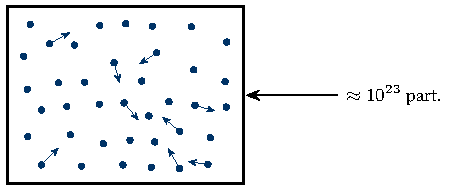
\includegraphics{figuras/gas-recipiente.pdf}
\end{figure}
Consideremos un gas contenido en un recipiente. En esta perspectiva, podemos ver que el sistema
está formado por un gran número de partículas (átomos o moléculas). Como ya sabemos, este número
debe ser proporcional a los moles del sistema y, por lo tanto, proporcional al número de Avogadro
($6.0221\times10^{23}$ partículas).

\begin{observacion}
  El \emph{número de Avogadro} es el número de partículas micro (átomos o moléculas) en 1~mol de
  dicha sustancia. Por ejemplo, 1~mol de H$\,\approx\,1$~g de H y 1~mol de $\mathrm{C}_{12}$
  $\approx\,12$~g de $\mathrm{C}_{12}$.
\end{observacion}

Para poder describir un sistema desde el punto de vista microscópico deberíamos describir el
comportamiento de cada una de las partículas que forman el sistema. Esto implica encontrar las
\emph{ecuaciones de movimiento} de cada una de ellas:
\begin{align*}
  \vec{x}_1 &= \vec{x}_1(t),\\
  \vec{x}_2 &= \vec{x}_2(t),\\
  &\;\;\vdots\\
  \vec{x}_j &= \vec{x}_j(t),
\end{align*}
donde, en coordenadas cartesianas,
\begin{equation*}
  \vec{x}_j(t)=\bigl(x_j(t),\,y_j(t),\,z_j(t)\bigr)
  \quad\Longrightarrow\quad
  \vec{x}_j(t)=x_j(t)\,\hat{e}_x+y_j(t)\,\hat{e}_y+z_j(t)\,\hat{e}_z.
\end{equation*}
Por lo tanto, hay que encontrar del orden de $10^{23}$ ecuaciones de movimiento, normalmente a
partir de resolver ecuaciones diferenciales. Además, estas partículas pueden interactuar entre sí
a través de colisiones o fuerzas causadas por campos de interacción. Se deberían entonces resolver
$10^{23}$ ecuaciones diferenciales acopladas, lo que evidentemente sigue siendo inviable.

Para poder hacer una descripción microscópica de un sistema termodinámico se ha desarrollado otra
teoría, que en este momento no es relevante.
\begin{equation*}
  \begin{gathered}\text{Sistema termodinámico (descripción micro)}\\\Longleftrightarrow\ \text{muchos parámetros relevantes con sus componentes micro.}\end{gathered}
\end{equation*}

\subsection*{Descripción microscópica vs.\ macroscópica}

A primera vista ambas descripciones parecen ser incompatibles y muy diferentes entre sí; sin
embargo, ambas deberían ser equivalentes para poder describir adecuadamente a los sistemas
termodinámicos.

En este momento no estamos interesados en estudiar la descripción microscópica, pero es
interesante pensar en que las variables macroscópicas (llamadas \textbf{variables termodinámicas}
o \textbf{coordenadas termodinámicas}) deben relacionarse de alguna forma con las cantidades
microscópicas.

\begin{modelo}[Postura de este curso]
  En este curso se considerará que las $10^{23}$ ecuaciones de movimiento son irrelevantes a nivel
  macroscópico y que las pocas variables macro (\emph{variables de bulto}) son las únicas
  relevantes para describir al sistema termodinámico.
\end{modelo}

La simplicidad de la descripción macroscópica y la elección de las posibles variables
termodinámicas para describir a un sistema termodinámico radica en dos propiedades de las
mediciones macroscópicas:
\begin{enumerate}[label=\arabic*.,itemsep=0pt]
  \item Las medidas macroscópicas son extremadamente \emph{lentas} comparadas con la escala
    atómica/molecular.
  \item Las medidas macroscópicas son extremadamente \emph{burdas} en las escalas de tamaños
    atómicos o moleculares.
\end{enumerate}
Es decir, la dinámica micro (movimientos rápidos y complejos) corresponde a una medición macro
lenta y burda.

De todas las posibles coordenadas microscópicas que describen al sistema durante una medición,
solo unas pocas combinaciones de ellas, que son prácticamente independientes del tiempo, son
observables macroscópicamente. Una medición macro (las mejores rondan $10^{-7}\,\mathrm{s}$) es
mucho más lenta que los procesos microscópicos (del orden de $10^{-15}\,\mathrm{s}$).
% VERIFICAR: exponentes 10^{-7} y 10^{-15} (manuscrito poco claro).
Es sensato considerar entonces que el caso macro representa un caso límite, para el cual se
construye una teoría de fenómenos independientes del tiempo; dicha teoría es la termodinámica.

\begin{definicion}[Alcance de la termodinámica]
  La termodinámica describe \textbf{únicamente estados estáticos} de los sistemas macroscópicos.
\end{definicion}

Además, las cantidades sujetas a principios de conservación (que no varían en el tiempo) son los
candidatos más obvios a ser variables termodinámicas:
\begin{itemize}[itemsep=0pt]
  \item energía,
  \item momento,
  \item momento angular,
  \item campo magnético;
\end{itemize}
pero hay otras.

Podemos entonces delimitar los objetivos de la termodinámica del siguiente modo:
\begin{quote}
  <<La termodinámica se encarga de estudiar las consecuencias \emph{macroscópicas} del gran número
  de grados de libertad microscópicos (atómicos o moleculares), las cuales, en virtud de lo burdo
  de las mediciones macroscópicas, no aparecen explícitamente en la descripción macroscópica del
  sistema.>>
\end{quote}

\section{Tipos de fronteras. Variables intensivas y extensivas}

\subsection*{La composición de los sistemas termodinámicos}

La termodinámica es un tema de gran generalidad y es aplicable a sistemas con una estructura
elaborada, con todo tipo de propiedades complejas del tipo mecánico, eléctrico, térmico, etc.
Por el momento estamos interesados en las \emph{propiedades térmicas}.

Para tal propósito es conveniente restringir por el momento nuestro estudio a sistemas
termodinámicos cuyas propiedades mecánicas y eléctricas sean ideales y simplificadas. En
analogía, simplificaciones del tipo:
\begin{enumerate}[label=\alph*),itemsep=0pt]
  \item péndulo simple (ideal) $\to$ péndulo físico (momento de inercia, disipativo, etc.);
  \item oscilador armónico simple (ideal) $\to$ oscilador (forzado, amortiguado).
\end{enumerate}

Por el momento restringiremos nuestra atención a los llamados \emph{sistemas termodinámicos
simples}, los cuales definimos a continuación.

\begin{definicion}[Sistema termodinámico simple]
  Es aquel sistema que es macroscópicamente homogéneo (simetría ante traslaciones), isotrópico
  (simetría ante rotaciones), eléctricamente neutro, suficientemente grande para evitar efectos
  superficiales (como la tensión superficial) y sobre el cual \textbf{no} actúan campos
  eléctricos, magnéticos ni gravitacionales.
\end{definicion}

Para este tipo de sistemas:
\begin{itemize}[itemsep=0pt]
  \item no hay ninguna coordenada eléctrica;
  \item no hay momentos eléctricos (monopolo, dipolo, cuadrupolo);
  \item las componentes del tensor de esfuerzos elásticos son cero.
\end{itemize}

\subsection*{Tipos de sistemas según su frontera}

Antes de proseguir con las coordenadas termodinámicas relevantes es importante discutir los tipos
de sistemas termodinámicos en función del \emph{tipo de frontera} que delimitan no solo al
sistema del resto del universo, sino cómo interactúa dicho sistema con el resto del universo (es
decir, cómo ocurre el intercambio de materia y energía entre el sistema y el universo). Hay tres
tipos de sistemas clasificados por el tipo de frontera:

\begin{definicion}[Sistema aislado]
  Son aquellos sistemas que no intercambian materia ni energía con el exterior.
\end{definicion}

Estos sistemas no existen en la naturaleza y solo se pueden considerar como sistemas aislados
aquellos que intercambian energía y materia con el universo de forma muy lenta. De hecho, el
único sistema aislado real es el universo mismo.

\begin{definicion}[Sistema cerrado]
  Son aquellos sistemas que intercambian energía pero no materia con el exterior.
\end{definicion}

Por ejemplo, un matraz con químicos en reacción mantenido a temperatura constante es un sistema
cerrado.

\begin{definicion}[Sistema abierto]
  Son aquellos que llevan a cabo intercambio de materia y energía con el exterior.
\end{definicion}

Por ejemplo, todos los seres vivos son sistemas abiertos.

\begin{figure}[H]
  \centering
  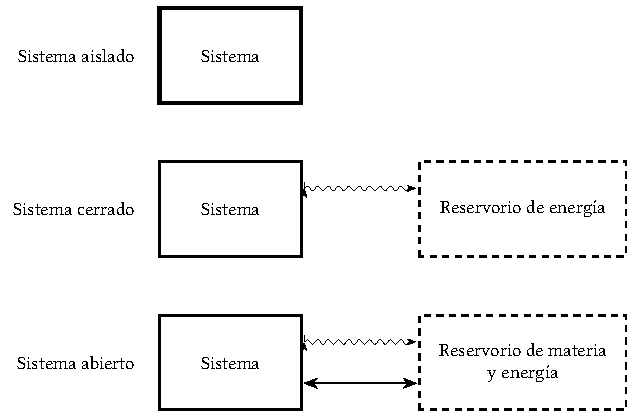
\includegraphics{figuras/tipos-sistemas.pdf}
\end{figure}

\subsection*{Paredes y restricciones}

Otro ingrediente fundamental en la descripción de los sistemas termodinámicos son las
especificaciones de las paredes (fronteras) que separan a un sistema del resto del universo, ya
que a través de las manipulaciones a estas paredes se generan procesos que alteran los parámetros
del sistema al redistribuirlos. Estas paredes se clasifican de acuerdo con aquellas propiedades que
dichas paredes pueden o no permitir su redistribución.

\begin{ejemplo}
  Dos sistemas (gas 1 con $U_1,V_1,N_1$ y gas 2 con $U_2,V_2,N_2$) colocados dentro de un cilindro
  rígido, separados por un pistón interno (pared, frontera). El sistema conjunto es cerrado, de modo
  que $V_1+V_2=V$ y $V_1'+V_2'=V$. Si el pistón está fijo, entonces no se permite el cambio del
  volumen, mientras que si es móvil, los volúmenes pueden cambiar:
  \begin{itemize}[itemsep=0pt]
    \item pistón fijo $=$ restricción ante cambios de $V$;
    \item pistón móvil $=$ permite cambios de $V$.
  \end{itemize}
  Por lo tanto, pistón fijo $\Rightarrow V_1=V_1',\ V_2=V_2'$ siempre, y pistón móvil
  $\Rightarrow V_1\neq V_1',\ V_2\neq V_2'$ en general.
  \begin{figure}[H]
    \centering
    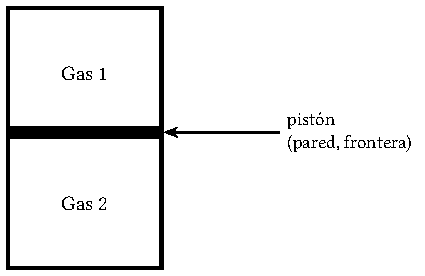
\includegraphics{figuras/cilindro-pistones.pdf}
  \end{figure}
\end{ejemplo}

\begin{definicion}[Pared móvil y pared rígida]
  Una pared que permite cambios en el volumen es llamada \textbf{pared móvil}, mientras que una
  pared que no permite cambios de volumen es llamada \textbf{pared rígida}.
\end{definicion}

Similarmente, podemos clasificar otras paredes de acuerdo con el tipo de restricción o
reordenamiento de los parámetros termodinámicos. Entre ellas tenemos:
\begin{itemize}[itemsep=0pt]
  \item \textbf{Pared adiabática:} no permite el intercambio de calor.
  \item \textbf{Pared diatérmica:} permite el intercambio de calor.
  \item \textbf{Pared permeable:} permite el paso de materia.
  \item \textbf{Pared impermeable:} no permite el paso de materia.
\end{itemize}

También hay paredes \textbf{semipermeables}, que permiten el flujo solo de tipos de materia
específicos (piensen, por ejemplo, en un filtro de café).

Así, el \textbf{equilibrio térmico} es aquel estado alcanzado por dos o más sistemas, caracterizado
por un número restringido de valores de las coordenadas del sistema, después de estar en
comunicación a través de una pared diatérmica.

Entonces, una pared que no permite el flujo del calor (que aún no hemos definido) es una pared
adiabática; pensemos, por ejemplo, en una hielera. Si además no permite el flujo de trabajo sobre
el sistema (como puede ser agitar una mezcla de agua con hielo), dichas paredes son
\emph{restrictivas respecto de la energía}. Por lo tanto, \textbf{la energía debe ser
macroscópicamente controlable}.

Otro aspecto importante es la forma en la que se mide la energía. Consideremos un sistema cerrado
$(U,V,N)\to(U',V',N)$ separado por paredes adiabáticas con un pistón móvil, el cual, por acción
de un agente externo, se puede mover para expandir o contraer el sistema.
\begin{figure}[H]
  \centering
  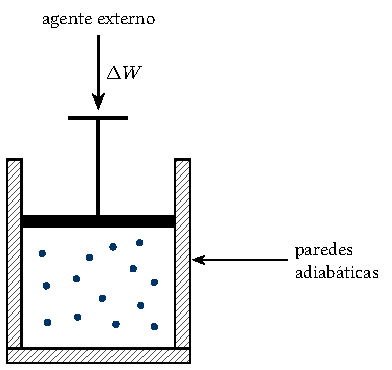
\includegraphics{figuras/trabajo-adiabatico.pdf}
\end{figure}
El agente externo ejerce un trabajo (bien definido) sobre el sistema, de modo que solo hay procesos
mecánicos actuando sobre el sistema. En esta situación, ya que el trabajo es lo único que se puede
variar en términos de la energía, entre dos estados dados las únicas diferencias de energía
posibles son los cambios en el trabajo mecánico, si el sistema está rodeado de paredes
adiabáticas.

\begin{postulado}[Trabajo adiabático]
  Existen paredes, llamadas adiabáticas, con la propiedad de que el trabajo hecho para llevar al
  sistema cerrado adiabáticamente del estado $A$ al estado $B$ es determinado únicamente por los
  estados, independientemente de todas las condiciones externas. El trabajo hecho es la diferencia
  en la energía interna de los dos estados.
\end{postulado}

\subsection*{Parámetros macroscópicos de un sistema simple}

Regresando a los sistemas simples, el \textbf{volumen} $V$ del sistema permanece como un
parámetro mecánico relevante. Asimismo, un sistema simple debe tener una composición química bien
definida, la cual debe estar descrita por un conjunto de parámetros adecuados.

\begin{figure}[H]
  \centering
  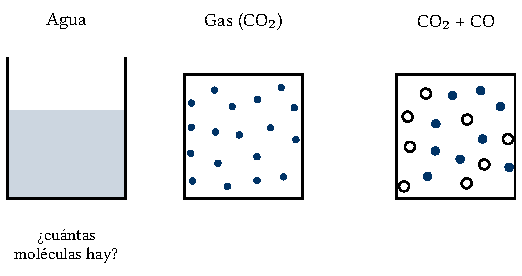
\includegraphics{figuras/composicion.pdf}
\end{figure}
Una forma razonable de construir el conjunto de parámetros que describen la composición química es
relacionarlo con el número total de moléculas o partículas que lo forman, ya sea una sustancia
pura o una mezcla de diferentes tipos de sustancia. Al ser un sistema macroscópico, resulta más
conveniente describirlo en términos del \textbf{número de moles} $N$ de la sustancia en cuestión.
Por lo tanto:
\begin{enumerate}[label=\arabic*.,itemsep=2pt]
  \item Para una sustancia \textbf{monocomponente}, la descripción química será proporcionada por el
    número de moles $N$ de la sustancia en el sistema. Por ejemplo, si el sistema está formado por
    $\mathrm{H_2O}$, con $N=10$ moles, la masa del sistema será de $180.15$ gramos de esta
    sustancia.
  \item Para un sistema \textbf{multicomponente} (formado, como por mezcla, de $K$ diferentes
    sustancias) éste será descrito por un número de moles para cada una de ellas, denotadas por
    $N_i$ con $i=1,2,3,\dots,K$. Por ejemplo, una mezcla de $\mathrm{CO_2}$ con $N_1=5$ moles y CO
    con $N_2=5$ moles tiene una masa de $m_1=220.045$~g $+\,m_2=140.050$~g, es decir,
    $m_T=360.095$~g, para $N=10$ moles en total.
    % VERIFICAR: masas 220.045 y 140.050 (transcripción del manuscrito).
\end{enumerate}

Si un sistema es una mezcla de $K$ componentes químicos, las $K$ razones
\begin{equation*}
  \frac{N_i}{\displaystyle\sum_{j=1}^{K}N_j}\qquad(i=1,2,3,\dots,K)
\end{equation*}
son llamadas \textbf{fracciones molares}. Además,
\begin{equation*}
  \sum_{i=1}^{K}\frac{N_i}{\displaystyle\sum_{j=1}^{K}N_j}=1.
\end{equation*}
Asimismo, $\displaystyle V\Big/\sum_{j=1}^{K}N_j$ es llamado \textbf{volumen molar}.

\subsubsection*{Parámetros extensivos}

Los parámetros macroscópicos $V,N_1,N_2,\dots,N_K$ tienen una propiedad importante. Si se tienen
dos sistemas idénticos, cada uno con volumen $V$ y moles $N_i$, y se unen para formar un sistema
nuevo, el volumen y el número de moles es el doble de los sistemas originales:
\begin{equation*}
  (V,\,N_i)\;+\;(V,\,N_i)\;=\;(2V,\,2N_i).
\end{equation*}
\begin{figure}[H]
  \centering
  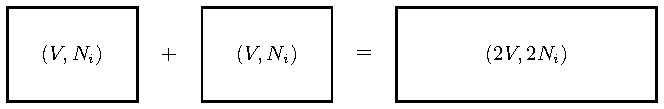
\includegraphics{figuras/extensivos-V.pdf}
\end{figure}
Cuando esto ocurre, se dice que estos parámetros son llamados \textbf{parámetros extensivos}, los
cuales son muy importantes en termodinámica.

\subsection*{Parámetros intensivos}

Ya que estamos interesados en estudiar sistemas, procesos y los cambios asociados de los parámetros
extensivos, nos interesa trabajar con la forma diferencial de la relación fundamental. Tomando la
representación energética de la relación fundamental, es decir, $U(S,V,N_1,\dots,N_r)$, su primer
diferencial es (recordemos que para $f=f(x,y)$, $\dd f=\pdv{f}{x}\dd x+\pdv{f}{y}\dd y$):
\begin{equation*}
  \dd U=\pdvc{U}{S}{V,N_1,\dots,N_r}\dd S+\pdvc{U}{V}{S,N_1,\dots,N_r}\dd V
  +\sum_{i=1}^{r}\pdvc{U}{N_i}{S,V,N_1,\dots,N_{i-1},N_{i+1},\dots,N_r}\dd N_i.
\end{equation*}
Dada la relevancia de las derivadas parciales en esta expresión, es conveniente denotarlas usando
símbolos específicos.

\begin{definicion}[Parámetros intensivos]
  \begin{align*}
    T&\equiv\pdvc{U}{S}{V,N_1,\dots,N_r}\quad\text{(temperatura)},\\
    P&\equiv-\pdvc{U}{V}{S,N_1,\dots,N_r}\quad\text{(presión)},\\
    \mu_i&\equiv\pdvc{U}{N_i}{S,V,N_1,\dots,N_{i-1},N_{i+1},\dots,N_r}\quad\text{(potencial electroquímico del $i$-ésimo componente molar)}.
  \end{align*}
  Estos parámetros son llamados \textbf{parámetros intensivos} ya que son independientes del tamaño
  del sistema.
\end{definicion}

$\mu_i$, el potencial electroquímico (o potencial químico), es la energía libre por unidad de
cantidad de una sustancia (por mol, en este caso) que se asocia a la tendencia de las partículas a
fluir debido a las diferencias de concentración (difusión). Formalmente, también incluye la
contribución debida a las cargas eléctricas de las partículas al moverse en campos eléctricos, pero
esta contribución es, en general, muy pequeña.

Con estas definiciones, el cambio infinitesimal de la energía está dado por:
\begin{equation*}
  \dd U=T\,\dd S-P\,\dd V+\sum_{i=1}^{r}\mu_i\,\dd N_i.
\end{equation*}

Más adelante daremos definiciones formales para $T$ y $\mu$.

\section{Ecuación fundamental}

\subsection*{Relación fundamental termodinámica}

El problema central de la termodinámica puede ser entonces resuelto completamente con la ayuda del
\textbf{principio de máxima entropía}, si la entropía del sistema es una función conocida de los
parámetros extensivos,
\begin{equation*}
  S=S(U,V,N).
\end{equation*}
Esta función de los parámetros extensivos es conocida como \textbf{relación fundamental
termodinámica}.

Si la relación fundamental de un sistema termodinámico es conocida, entonces \emph{toda la
información termodinámica del sistema puede ser obtenida a partir de esta}.

\begin{postulado}[III]
  La entropía de un sistema compuesto es \textbf{aditiva} sobre sus subsistemas constitutivos. La
  entropía es continua y diferenciable y es una función monótonamente creciente de la energía.
\end{postulado}

De este postulado se siguen varias consecuencias matemáticas. Sea un sistema compuesto formado por
$\alpha$ subsistemas constitutivos.
\begin{figure}[H]
  \centering
  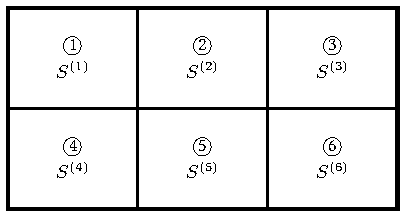
\includegraphics{figuras/seis-subsistemas.pdf}
\end{figure}
Entonces la entropía $S$ de este sistema será la suma de las entropías de cada uno de estos
subsistemas, es decir,
\begin{equation*}
  S=S^{(1)}+S^{(2)}+S^{(3)}+\cdots+S^{(\alpha)}=\sum_{i=1}^{\alpha}S^{(i)}.
\end{equation*}
Asimismo, de acuerdo con los postulados II y III, la entropía de cada uno de estos subsistemas es
una función \emph{únicamente} de los parámetros extensivos de ese subsistema:
\begin{equation*}
  S^{(j)}=S^{(j)}\bigl(U^{(j)},V^{(j)},N_1^{(j)},\dots,N_r^{(j)}\bigr)
  \qquad\text{para un sistema con $r$ tipos de partículas.}
\end{equation*}
Esto implica que la entropía de un subsistema no está afectada directamente por los otros
subsistemas.

La aditividad de $S$ tiene una implicación importante respecto a subsistemas espacialmente
separados:

\begin{proposicion}[Homogeneidad de la entropía]
  La entropía de un sistema simple es una función homogénea de orden uno de los parámetros
  extensivos.
\end{proposicion}

Para ver cómo se deriva esto, recordemos la definición de función homogénea de orden $n$.

\begin{definicion}[Función homogénea]
  Sea $f=f(x_1,x_2,\dots,x_m)$ una función de $m$ variables. Se dice que $f$ es \textbf{homogénea
  de orden $n$} si al escalar todos sus argumentos por un factor $\lambda>0$ la función se escala
  por $\lambda^{n}$; es decir,
  \begin{equation*}
    f(\lambda x_1,\lambda x_2,\dots,\lambda x_m)=\lambda^{n}f(x_1,x_2,\dots,x_m).
  \end{equation*}
\end{definicion}
% NOTA: en el manuscrito el factor aparece como "\lambda^n x_i" dentro de los argumentos; la definición correcta (usada aquí) es f(\lambda x_i)=\lambda^n f(x_i).

El caso de orden uno ocurre cuando $n=1$:
\begin{equation*}
  f(\lambda x_1,\lambda x_2,\dots,\lambda x_m)=\lambda f(x_1,x_2,\dots,x_m).
\end{equation*}
Por lo tanto, para el caso de la entropía se debe cumplir que
\begin{equation*}
  S(\lambda U,\lambda V,\lambda N_1,\lambda N_2,\dots,\lambda N_r)=\lambda\,S(U,V,N_1,N_2,\dots,N_r).
\end{equation*}

¿Cómo se deriva esto de la aditividad de la entropía de un sistema compuesto,
$S=S^{(1)}+S^{(2)}$? La relación se da a través del parámetro $\lambda$; por ejemplo, si $S^{(1)}$ y
$S^{(2)}$ son idénticos:
\begin{align*}
  S&=S^{(1)}(U,V,N_1,\dots,N_r)+S^{(1)}(U,V,N_1,\dots,N_r)\\
   &=S^{(1)}(2U,2V,2N_1,\dots,2N_r)=2\,S^{(1)}(U,V,N_1,\dots,N_r).
\end{align*}
Es decir, en este caso $\lambda=2$. Por lo que, si el sistema compuesto está formado por dos
subsistemas idénticos, entonces los valores de $U,V,N_1,\dots,N_r$ se duplican, justo como habíamos
explicado previamente.

Asimismo, otra consecuencia del postulado III es la siguiente. Al ser una función monótonamente
creciente de la energía interna $U$, la entropía $S$ aumenta cuando $U$ aumenta; matemáticamente
esto puede escribirse, para cambios infinitesimales de la energía, como
\begin{equation*}
  \lim_{\Delta U\to0}\frac{\Delta S}{\Delta U}=\pdvc{S}{U}{V,N_1,\dots,N_r}>0,
\end{equation*}
donde los subíndices indican que $V,N_1,\dots,N_r$ se mantienen constantes. Esto tiene una relación
con la temperatura $T$ que exploraremos más adelante ($T\geq0$).

Otras consecuencias importantes desde el punto de vista matemático son las siguientes. La
continuidad, diferenciabilidad y monotonía de la entropía implican que la entropía puede ser
invertida con respecto a la energía, y la energía es una función \emph{univaluada} ($U$ solo puede
tomar un valor por cada valor de $S$), continua y diferenciable de $S,V,N_1,\dots,N_r$. Es decir,
la función $S=S(U,V,N_1,\dots,N_r)$ puede ser resuelta unívocamente para $U$ de la forma
\begin{equation*}
  U=U(S,V,N_1,\dots,N_r).
\end{equation*}

¿Por qué estas propiedades derivan en esta consecuencia?
\begin{enumerate}[label=\arabic*.,itemsep=3pt]
  \item \textbf{Continuidad.} No hay saltos ni discontinuidades en $S(U)$; de forma que existe una
    relación funcional bien definida en todo el dominio de definición de $S$.
  \item \textbf{Diferenciabilidad.} Implica que las derivadas de $S$ respecto de los parámetros
    existen; y si además estas derivadas no se anulan, implica que se puede aplicar el teorema de
    la función inversa, el cual establece que esta puede invertirse localmente.
  \item \textbf{Monótonamente creciente.} Ya vimos que esto implica que $\partial S/\partial U>0$, lo
    que implica que es una función inyectiva (es decir, no toma el mismo valor dos veces); esta es
    una condición necesaria para que $S$ sea invertible globalmente.
\end{enumerate}

Por lo tanto, las formas $S=S(U,V,N_1,\dots,N_r)$ y $U=U(S,V,N_1,\dots,N_r)$ son formas
alternativas de la relación fundamental, por lo que ambas contienen toda la información
termodinámica del sistema.
% NOTA: en el manuscrito la segunda forma se escribe "U=U(U,V,N_1,...,N_r)"; por el contexto es U(S,V,N_1,...,N_r).

Otra consecuencia de las propiedades de la entropía es que, gracias a la extensividad de $S$, es
posible escalar las propiedades de un sistema de $N$ moles a partir de las propiedades de un sistema
de $1$ mol:
\begin{equation*}
  S(U,V,N_1,N_2,\dots,N_r)=N\,S\!\left(\frac{U}{N},\frac{V}{N},\frac{N_1}{N},\frac{N_2}{N},\dots,\frac{N_r}{N}\right),
\end{equation*}
donde $N=\sum_{k=1}^{r}N_k$ es el número total de moles, y se toma $\lambda=1/N$ en la
homogeneidad de orden uno.
% NOTA: en el manuscrito la constante de escala aparece escrita como "\lambda = N/N = N\cdot 1/\sum N_k"; se interpretó como \lambda=1/N=1/\sum_k N_k.

Para un sistema simple monocomponente (un solo tipo de sustancia),
\begin{equation*}
  S(U,V,N)=N\,S\!\left(\frac{U}{N},\frac{V}{N},1\right),
\end{equation*}
con $u\equiv U/N$ la \textbf{energía interna reducida} (o energía interna por mol) y
$v\equiv V/N$ el \textbf{volumen reducido} (o volumen por mol).

De aquí, $S\!\left(\frac{U}{N},\frac{V}{N},1\right)=S(u,v,1)$ es la entropía de un sistema de $1$ mol,
y es usual utilizar la notación $s(u,v)\equiv S(u,v,1)$, de manera que
\begin{equation*}
  S(U,V,N)=N\,s(u,v).
\end{equation*}

\subsection*{Ecuación de Euler}

Veamos ahora algunas propiedades matemáticas de la relación fundamental. Partiendo de la definición
de la homogeneidad de primer orden de $U(S,V,N_1,\dots,N_r)$,
\begin{equation*}
  U(\lambda S,\lambda X_1,\dots,\lambda X_t)=\lambda\,U(S,X_1,\dots,X_t),
\end{equation*}
con $X_1=V$, $X_2=N_1,\dots,X_t=N_r$; si se diferencia esta relación respecto a $\lambda$, se obtiene
\begin{align*}
  \pdv{\lambda}\Bigl[U(\lambda S,\lambda X_1,\dots,\lambda X_t)\Bigr]&=\pdv{\lambda}\Bigl[\lambda\,U(S,X_1,\dots,X_t)\Bigr]\\
  \Longrightarrow\quad\pdv{U}{(\lambda S)}\pdv{(\lambda S)}{\lambda}+\pdv{U}{(\lambda X_1)}\pdv{(\lambda X_1)}{\lambda}+\cdots+\pdv{U}{(\lambda X_t)}\pdv{(\lambda X_t)}{\lambda}&=U(S,X_1,\dots,X_t)\\
  \text{o bien}\quad\pdv{U}{(\lambda S)}\,S+\sum_{j=1}^{t}\pdv{U}{(\lambda X_j)}\,X_j&=U(S,X_1,\dots,X_t).
\end{align*}
Ya que esta relación es en general cierta para todo $\lambda$, consideremos el caso particular
$\lambda=1$; se obtiene
\begin{equation*}
  \pdv{U}{S}\,S+\sum_{j=1}^{t}\pdv{U}{X_j}\,X_j=U;
\end{equation*}
sustituyendo las derivadas con $P_1=-\pdv{U}{V}$, $P_2=\pdv{U}{N_1},\dots$,
\begin{equation*}
  \boxed{U=TS+\sum_{j=1}^{t}P_jX_j}
\end{equation*}
Para un sistema simple en particular se tiene
\begin{equation*}
  \boxed{U=TS-PV+\mu_1N_1+\mu_2N_2+\cdots+\mu_rN_r}
\end{equation*}
Esta relación es llamada \textbf{ecuación de Euler}.

En la representación entrópica, $S=\sum_{j=0}^{t}F_jX_j$ (con $X_0=U$), o bien
\begin{equation*}
  S=\left(\frac{1}{T}\right)U+\left(\frac{P}{T}\right)V-\sum_{k=1}^{r}\left(\frac{\mu_k}{T}\right)N_k.
\end{equation*}

\subsection*{Relación de Gibbs--Duhem}

Las condiciones de equilibrio nos permiten encontrar relaciones entre los parámetros intensivos (en
el caso de un sistema simple, entre $T$, $P$, $\mu$). Aunque es posible introducir algunos
parámetros (como $T$ o $P$) debido a la noción intuitiva que se tiene de estos, y a pesar de no
tener alguna noción intuitiva de otros parámetros intensivos (como el caso de $\mu$), es posible
introducir el resto de parámetros intensivos de la teoría de modo similar, por lo que la teoría es
\emph{simétrica} en los parámetros intensivos.

Sin embargo, es importante notar que no todos los parámetros intensivos son independientes entre sí;
existe una relación entre parámetros intensivos, y en el caso particular de un sistema simple
monocomponente, $\mu$ puede ser escrito como una función de $T$ y $P$. La existencia de una
relación entre varios parámetros intensivos también es una consecuencia de que la relación
fundamental es homogénea de orden uno.

\begin{observacion}
  Para sistemas simples monocomponentes, esta propiedad permite que la relación fundamental pueda
  ser escrita de la forma $U=u(s,v)$, tal y como cuando se introdujeron las variables molares.
  Asimismo, cada uno de los tres parámetros intensivos es a su vez función de $s$ y $v$. Eliminar
  ambas de las tres ecuaciones de estado nos lleva a una relación entre $T$, $P$ y $\mu$.
\end{observacion}

Para sistemas más generales se puede hacer una extensión para encontrar una relación general.
Supongamos que se tiene una relación fundamental con $(t+1)$ variables extensivas,
$U=U(S,X_1,X_2,\dots,X_t)$, para las cuales hay $(t+1)$ ecuaciones de estado
\begin{equation*}
  P_k=P_k(S,X_1,X_2,\dots,X_t),\qquad P_i\equiv\pdv{U}{X_i},
\end{equation*}
con $P_1=-P$, $P_2=\mu_1$, $P_3=\mu_2,\dots$
% NOTA: en el manuscrito aparece "X_1=-P, X_2=\mu_1, X_3=\mu_2"; por el contexto son los parámetros intensivos P_1=-P, P_2=\mu_1, P_3=\mu_2.
las cuales son ecuaciones homogéneas de orden cero:
\begin{equation*}
  P_k(\lambda S,\lambda X_1,\dots,\lambda X_t)=P_k(S,X_1,X_2,\dots,X_t).
\end{equation*}
Si se escoge el parámetro $\lambda=1/X_t$, se tiene
\begin{equation*}
  P_k=P_k\!\left(\frac{S}{X_t},\frac{X_1}{X_t},\dots,\frac{X_{t-1}}{X_t},\frac{X_t}{X_t}\right)
  =P_k\!\left(\frac{S}{X_t},\frac{X_1}{X_t},\dots,\frac{X_{t-1}}{X_t},1\right).
\end{equation*}
De manera que cada uno de los $(t+1)$ parámetros intensivos es función de solo $t$ variables
termodinámicas de la forma $X_i/X_t$. La eliminación de las $t$ variables de entre las
$(t+1)$ ecuaciones nos da la relación que se busca entre los parámetros intensivos.

Conocer la relación funcional explícita que existe entre el conjunto de parámetros intensivos
requiere del conocimiento explícito de la relación fundamental del sistema y varía de sistema en
sistema.

Una forma diferencial entre los parámetros intensivos puede ser obtenida directamente a partir de
la ecuación de Euler, y es conocida como \textbf{relación de Gibbs--Duhem}. Partiendo de la ecuación
de Euler, $U=TS+\sum_{j=1}^{t}P_jX_j$, tomando la variación infinitesimal,
\begin{equation*}
  \dd U=T\,\dd S+S\,\dd T+\sum_{j=1}^{t}\bigl[P_j\,\dd X_j+X_j\,\dd P_j\bigr],
\end{equation*}
pero de acuerdo con la primera ley los cambios en la energía interna son
$\dd U=T\,\dd S-P\,\dd V+\mu_1\dd N_1+\cdots+\mu_r\dd N_r$, o bien $\dd U=T\,\dd S+\sum_{j=1}^{t}P_j\,\dd X_j$.
% NOTA: el manuscrito escribe "+P dV" en la primera forma; con P_1=-P el término es -P dV (coincide con la forma compacta).
Sustituyendo en la relación anterior,
\begin{equation*}
  T\,\dd S+\sum_{j=1}^{t}P_j\,\dd X_j=T\,\dd S+S\,\dd T+\sum_{j=1}^{t}P_j\,\dd X_j+\sum_{j=1}^{t}X_j\,\dd P_j,
\end{equation*}
de donde
\begin{equation*}
  \boxed{S\,\dd T+\sum_{j=1}^{t}X_j\,\dd P_j=0}\qquad\text{(relación de Gibbs--Duhem)}
\end{equation*}
Para un sistema de un solo componente se tiene
\begin{equation*}
  S\,\dd T-V\,\dd P+N\,\dd\mu=0,
  \qquad\text{o en coordenadas molares}\qquad
  \boxed{\dd\mu=-s\,\dd T+v\,\dd P}
\end{equation*}
Por lo tanto, la variación del potencial químico $\mu$ no es independiente de los cambios en $T$ y
$P$, pero los cambios en cualquiera de ellos pueden ser calculados en términos de los otros dos.

La relación de Gibbs--Duhem nos da una relación entre los parámetros intensivos en forma
diferencial. Si se integra esta ecuación en forma explícita, permite recuperar la relación
fundamental, pero solo si se conocen las ecuaciones de estado, que nos permiten obtener a los
parámetros extensivos en términos de los intensivos y viceversa. Entonces,
\begin{equation*}
  \underbrace{\text{Relación fundamental}}_{\text{(explícita)}}\;\equiv\;\underbrace{\text{Ecuaciones de estado}}_{\text{(conocer todas ellas)}}
  \qquad\text{[toda la información termodinámica del sistema]}.
\end{equation*}

En la representación entrópica se puede obtener una forma de la ecuación de Gibbs--Duhem (se deja
como ejercicio):
\begin{equation*}
  U\,\dd\!\left(\frac{1}{T}\right)+V\,\dd\!\left(\frac{P}{T}\right)-\sum_{k=1}^{r}N_k\,\dd\!\left(\frac{\mu_k}{T}\right)=0,
  \qquad\text{bajo la eliminación de}\qquad
  \sum_{j=0}^{t}X_j\,\dd F_j=0.
\end{equation*}

El número de parámetros intensivos independientes es llamado el \textbf{número de grados de
libertad termodinámicos}. Para un sistema simple monocomponente el número de grados de libertad es
$2$. Para un sistema con $r+1$ parámetros intensivos se tendrán entonces $r$ grados de libertad
termodinámicos y $r-1$ potenciales químicos independientes.
% NOTA: el manuscrito dice "t parámetros intensivos ... t-1 grados de libertad" con "r+1" escrito encima de "t" (t=r+1) y "r-1 potenciales químicos independientes".
Además, la relación define una hipersuperficie en el espacio termodinámico que conecta vectores
tangentes asociados con los cambios en $T$, $P$ y $\mu_i$.
\begin{figure}[H]
  \centering
  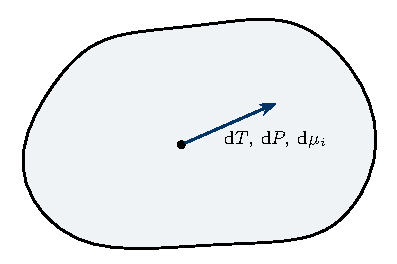
\includegraphics{figuras/hipersuperficie-tangente.pdf}
\end{figure}

Sea $U=U(S,V,N)$, lo cual implica
\begin{equation*}
  T(S,V,N)=T(s,v),\qquad P(S,V,N)=P(s,v),\qquad\mu(S,V,N)=\mu(s,v).
\end{equation*}
Si se conocen las tres ecuaciones de estado, se pueden sustituir en la relación de Euler y obtener
$U(S,V,N)$. Si se tienen dos ecuaciones de estado, se puede utilizar la ecuación de Gibbs--Duhem
para integrar y obtener la tercera, hasta una constante indeterminada.

Otro método para obtener la relación fundamental si se conocen dos ecuaciones de estado, y que suele
ser más directo y más conveniente en general, pero que es lógicamente equivalente a la ecuación de
Gibbs--Duhem, es la \emph{integración directa} de la relación molar,
\begin{equation*}
  \dd u=T\,\dd s-P\,\dd v,
\end{equation*}
ya que si se conocen $T=T(s,v)$ y $P=P(s,v)$, se obtiene una ecuación diferencial en tres variables
$u$, $s$ y $v$; al integrar o resolver dicha ecuación diferencial nos da
\begin{equation*}
  \boxed{u=u(s,v)}\quad\text{la relación fundamental.}
\end{equation*}

\begin{observacion}
  Siempre es posible expresar $U$ como función de otros parámetros que no sean $S,V,N$. Por ejemplo,
  se puede eliminar $S$ de $U=U(S,V,N)$ y $T=T(S,V,N)$ para obtener una relación de la forma
  $U=U(T,V,N)$; sin embargo, esta \textbf{no} es una relación fundamental y no contiene toda la
  información termodinámica del sistema.

  Además, la definición de $T\equiv\pdv{U}{S}$ implica que $U=U(T,V,N)$ en realidad es una ecuación
  diferencial parcial de $U$ en $S$; incluso si esta es integrable, dará una relación fundamental
  hasta algunas funciones indeterminadas. Por lo tanto,
  \begin{equation*}
    U=U(S,V,N)\;\Longrightarrow\;U=U(T,V,N)\qquad\text{pero}\qquad U=U(T,V,N)\;\not\Longrightarrow\;U=U(S,V,N),
  \end{equation*}
  por lo que la información contenida en ambas es diferente.
  \begin{figure}[H]
    \centering
    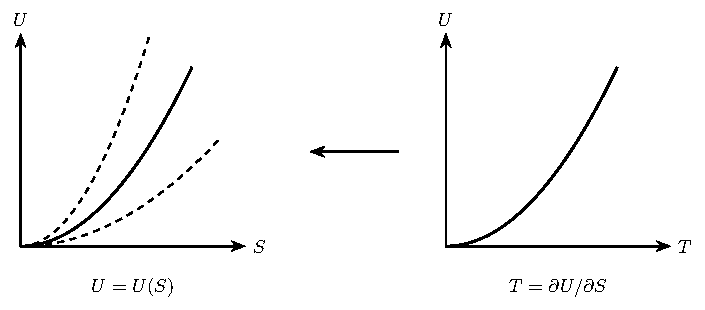
\includegraphics{figuras/U-S-T.pdf}
  \end{figure}
\end{observacion}

\section{Ecuaciones de estado}

\subsection*{Ecuaciones de estado}

Como $T$, $P$ y $\mu_i$ se definen como derivadas parciales de funciones de $S,V,N_1,\dots,N_r$,
también son funciones de estos parámetros, de manera que se tiene el conjunto de relaciones
funcionales de la forma
\begin{align*}
  T&=T(S,V,N_1,\dots,N_r),\\
  P&=P(S,V,N_1,\dots,N_r),\\
  \mu_i&=\mu_i(S,V,N_1,\dots,N_r),
\end{align*}
que son $r+2$ relaciones. Estas relaciones en términos de los parámetros extensivos independientes
son llamadas \textbf{ecuaciones de estado}. Conocer una sola ecuación de estado \emph{no}
constituye conocer toda la información termodinámica del sistema (posteriormente veremos que
conocer todas las ecuaciones de estado de un sistema equivale a conocer la ecuación fundamental).

Para un sistema monocomponente:
\begin{align*}
  U&=U(S,V,N)\quad(1\text{ relación fundamental}),\\
  T&=T(S,V,N),\quad P=P(S,V,N),\quad\mu=\mu(S,V,N)\quad(3\text{ ecuaciones de estado}).
\end{align*}
Geométricamente, estas relaciones se pueden entender como \emph{proyecciones} de la relación
fundamental.
\begin{figure}[H]
  \centering
  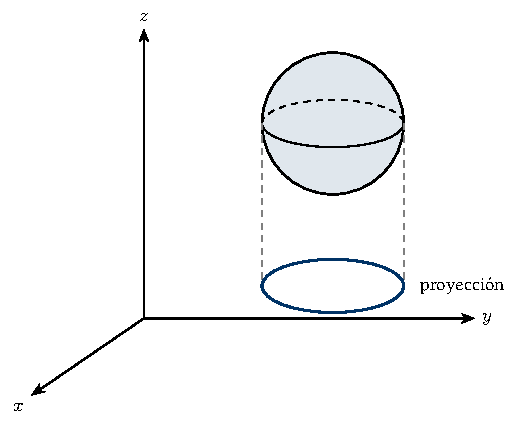
\includegraphics{figuras/esfera-proyeccion.pdf}
\end{figure}

\begin{proposicion}[Homogeneidad de las ecuaciones de estado]
  Ya que $U=U(S,V,N)$ es una función homogénea de orden $1$, las ecuaciones de estado son funciones
  homogéneas de orden cero.
\end{proposicion}

\begin{proof}
  Sea $f=f(x_1,\dots,x_n)$ tal que $f(\lambda x_1,\dots,\lambda x_n)=\lambda f(x_1,\dots,x_n)$, y
  definamos $g_i\equiv\pdv{f}{x_i}$, es decir, $g_i(x_1,\dots,x_n)=\pdv{f(x_1,\dots,x_n)}{x_i}$.
  Sustituyendo $x_j$ por $\lambda x_j$ para todo $j=1,\dots,n$,
  \begin{equation*}
    g_i(\lambda x_1,\dots,\lambda x_n)
    =\frac{\partial f(\lambda x_1,\dots,\lambda x_n)}{\partial(\lambda x_i)}
    =\frac{\partial\bigl[\lambda f(x_1,\dots,x_n)\bigr]}{\partial(\lambda x_i)}
    =\frac{\lambda\,\partial f(x_1,\dots,x_n)}{\lambda\,\partial x_i}
    =\frac{\partial f(x_1,\dots,x_n)}{\partial x_i},
  \end{equation*}
  como $\lambda$ es un parámetro constante. Por lo tanto,
  $g_i(\lambda x_1,\dots,\lambda x_n)=g_i(x_1,\dots,x_n)$, por lo que $g_i$ es una función
  homogénea de orden $0$.
\end{proof}

En particular,
\begin{equation*}
  T(\lambda S,\lambda V,\lambda N_1,\dots,\lambda N_r)=T(S,V,N_1,\dots,N_r),
\end{equation*}
por lo cual, y como se había discutido antes, estas relaciones son \emph{intensivas}: al ser
homogéneas de orden cero no son extensivas, ya que esto implica que son independientes del tamaño
del sistema. Por ejemplo, para $T$, la temperatura de una porción del sistema es la misma que la de
todo el sistema. Lo mismo ocurre con $P$ y $\mu$.

Una notación condensada para los parámetros extensivos e intensivos que se puede tomar es la
siguiente:
\begin{align*}
  V,N_1,\dots,N_r&\longrightarrow X_1,X_2,\dots,X_t\qquad(t=r+1),\\
  -P,\mu_1,\dots,\mu_r&\longrightarrow P_1,P_2,\dots,P_t\qquad(\text{con }P_1=-P),
\end{align*}
donde
\begin{align*}
  \pdvc{U}{S}{X_1,\dots,X_t}&\equiv T=T(S,X_1,X_2,\dots,X_t),\\
  \pdvc{U}{X_j}{S}&\equiv P_j=P_j(S,X_1,X_2,\dots,X_t),\qquad j=1,2,\dots,t,
\end{align*}
de modo que
\begin{equation*}
  \dd U=T\,\dd S+\sum_{j=1}^{t}P_j\,\dd X_j.
\end{equation*}

Para sistemas monocomponentes es común escribir $\dd U$ en términos de cantidades molares, de forma
similar a como se hizo con $S\to s$:
\begin{equation*}
  U(S,V,N)=N\,U\!\left(\frac{S}{N},\frac{V}{N},\frac{N}{N}\right)=N\,U(s,v,1)=N\,u(s,v),
\end{equation*}
con $u(s,v)\equiv U(s,v,1)$, $s=S/N$, $v=V/N$ y $u(s,v)=\frac{1}{N}U(S,V,N)$. De manera que
\begin{equation*}
  \dd u=\pdv{u}{s}\dd s+\pdv{u}{v}\dd v,\qquad
  \pdvc{u}{s}{v}=\pdvc{U}{S}{V,N}=T,\qquad
  \pdvc{u}{v}{s}=-P,
\end{equation*}
y por lo tanto
\begin{equation*}
  \dd u=T\,\dd s-P\,\dd v.
\end{equation*}

\subsubsection*{Ejercicios}

\begin{ejercicio}
  Encuentre las tres ecuaciones de estado del sistema con relación fundamental
  \begin{equation*}
    U=\left(\frac{v_0\theta}{R^{2}}\right)\frac{S^{3}}{NV}.
  \end{equation*}
\end{ejercicio}

\begin{solucion}
  Primero verificamos la homogeneidad de orden uno:
  \begin{equation*}
    U(\lambda S,\lambda V,\lambda N)=\left(\frac{v_0\theta}{R^{2}}\right)\frac{\lambda^{3}S^{3}}{(\lambda N)(\lambda V)}
    =\lambda\left(\frac{v_0\theta}{R^{2}}\right)\frac{S^{3}}{NV}=\lambda\,U(S,V,N).
  \end{equation*}
  Entonces:
  \begin{align*}
    \pdvc{U}{S}{V,N}&=3\left(\frac{v_0\theta}{R^{2}}\right)\frac{S^{2}}{NV}=T,\\
    \pdvc{U}{V}{S,N}&=-\left(\frac{v_0\theta}{R^{2}}\right)\frac{S^{3}}{NV^{2}}=-P
      \;\Longrightarrow\;P=\left(\frac{v_0\theta}{R^{2}}\right)\frac{S^{3}}{NV^{2}},\\
    \pdvc{U}{N}{S,V}&=-\left(\frac{v_0\theta}{R^{2}}\right)\frac{S^{3}}{N^{2}V}=\mu
      \;\Longrightarrow\;\mu=-\left(\frac{v_0\theta}{R^{2}}\right)\frac{S^{3}}{N^{2}V}.
  \end{align*}
  Como comprobación, las tres son homogéneas de orden cero:
  \begin{align*}
    T(\lambda S,\lambda V,\lambda N)&=3\left(\frac{v_0\theta}{R^{2}}\right)\frac{\lambda^{2}S^{2}}{\lambda^{2}NV}=T,\\
    P(\lambda S,\lambda V,\lambda N)&=\left(\frac{v_0\theta}{R^{2}}\right)\frac{\lambda^{3}S^{3}}{\lambda^{3}NV^{2}}=P,\\
    \mu(\lambda S,\lambda V,\lambda N)&=-\left(\frac{v_0\theta}{R^{2}}\right)\frac{\lambda^{3}S^{3}}{\lambda^{3}N^{2}V}=\mu.
  \end{align*}
\end{solucion}

\begin{ejercicio}
  Para el sistema del problema anterior, encuentre $\mu$ en función de $T$, $V$ y $N$.
\end{ejercicio}

\begin{solucion}
  Como ya se ha visto,
  \begin{equation*}
    T=3\left(\frac{v_0\theta}{R^{2}}\right)\frac{S^{2}}{NV}
    \qquad\text{y}\qquad
    \mu=-\left(\frac{v_0\theta}{R^{2}}\right)\frac{S^{3}}{N^{2}V},
  \end{equation*}
  entonces se debe eliminar $S$ y reemplazarla por $T$:
  \begin{equation*}
    \frac{1}{3}NVT\left(\frac{v_0\theta}{R^{2}}\right)^{-1}=S^{2}
    \quad\text{o}\quad
    S=\sqrt{\frac{1}{3}\left(\frac{R^{2}}{v_0\theta}\right)NVT}.
  \end{equation*}
  Sustituyendo en $\mu$,
  \begin{align*}
    \mu&=-\left(\frac{v_0\theta}{R^{2}}\right)\frac{1}{N^{2}V}\left[\frac{1}{3}\left(\frac{R^{2}}{v_0\theta}\right)NVT\right]^{3/2}
      =-\frac{v_0\theta}{R^{2}}\left(\frac{R^{2}}{v_0\theta}\right)^{3/2}\frac{\left(\frac{1}{3}NVT\right)^{3/2}}{N^{2}V}\\
    &=-\frac{R}{\sqrt{v_0\theta}}\left(\frac{1}{3}\right)^{3/2}\frac{V^{1/2}T^{3/2}}{N^{1/2}}
      =-R\left[\left(\frac{1}{3}\right)^{3}\frac{VT^{3}}{v_0\theta\,N}\right]^{1/2},
  \end{align*}
  de modo que $\mu=\mu(T,V,N)$. Esto \textbf{no} es una ecuación de estado.
\end{solucion}

\begin{ejercicio}
  Encuentre las tres ecuaciones de estado del sistema cuya relación fundamental molar es
  \begin{equation*}
    u=\left(\frac{v_0\theta}{R}\right)\frac{s^{2}}{v}\,e^{s/R}.
  \end{equation*}
\end{ejercicio}

\begin{solucion}
  Para calcular las ecuaciones de estado, escribamos esta relación en términos de $S$, $V$ y $N$:
  \begin{equation*}
    u=\left(\frac{v_0\theta}{R}\right)\left(\frac{S}{N}\right)^{2}\left(\frac{N}{V}\right)\exp\!\left[\frac{1}{R}\frac{S}{N}\right]
    =\left(\frac{v_0\theta}{R}\right)\frac{S^{2}}{NV}\exp\!\left[\frac{1}{R}\frac{S}{N}\right].
  \end{equation*}
  Como $\frac{1}{N}U(S,V,N)=u(s,v)$, se tiene $U(S,V,N)=N\,u$, es decir,
  \begin{equation*}
    U(S,V,N)=\left(\frac{v_0\theta}{R}\right)\frac{S^{2}}{V}\exp\!\left(\frac{1}{R}\frac{S}{N}\right),
  \end{equation*}
  y se verifica $U(\lambda S,\lambda V,\lambda N)=\left(\frac{v_0\theta}{R}\right)\frac{\lambda^{2}S^{2}}{\lambda V}\exp\!\left(\frac{1}{R}\frac{\lambda S}{\lambda N}\right)=\lambda\,U(S,V,N)$.
  Entonces:
  \begin{align*}
    T&=\pdvc{U}{S}{V,N}=\left(\frac{v_0\theta}{R}\right)\left[\frac{2S}{V}\exp\!\left(\frac{1}{R}\frac{S}{N}\right)+\frac{S^{2}}{V}\left(\frac{1}{R}\frac{1}{N}\right)\exp\!\left(\frac{1}{R}\frac{S}{N}\right)\right]\\
     &=\left(\frac{v_0\theta}{R}\right)\left[\frac{2S}{V}+\frac{1}{R}\frac{S^{2}}{NV}\right]\exp\!\left(\frac{1}{R}\frac{S}{N}\right),
  \end{align*}
  y $T(\lambda S,\lambda V,\lambda N)=T(S,V,N)$;
  \begin{align*}
    P&=-\pdvc{U}{V}{S,N}=-\left[-\left(\frac{v_0\theta}{R}\right)\frac{S^{2}}{V^{2}}\exp\!\left(\frac{1}{R}\frac{S}{N}\right)\right]
      =\left(\frac{v_0\theta}{R}\right)\frac{S^{2}}{V^{2}}\exp\!\left(\frac{1}{R}\frac{S}{N}\right),
  \end{align*}
  y $P(\lambda S,\lambda V,\lambda N)=P(S,V,N)$;
  \begin{align*}
    \mu&=\pdvc{U}{N}{S,V}=\left(\frac{v_0\theta}{R}\right)\frac{S^{2}}{V}\left(-\frac{1}{R}\frac{S}{N^{2}}\right)\exp\!\left(\frac{1}{R}\frac{S}{N}\right)
      =-\left(\frac{v_0\theta}{R^{2}}\right)\frac{S^{3}}{N^{2}V}\exp\!\left(\frac{1}{R}\frac{S}{N}\right),
  \end{align*}
  y $\mu(\lambda S,\lambda V,\lambda N)=\mu(S,V,N)$.
\end{solucion}

\subsection*{Parámetros intensivos entrópicos}

¿Qué ocurre si, en lugar de usar $U=U(S,V,N)$ como relación fundamental, utilizamos
$S=S(U,V,N)$? Ya establecimos que ambas representaciones son equivalentes, por lo que las
variaciones infinitesimales de la entropía, de acuerdo con la primera ley, deben dar un resultado
similar al caso de la energía interna. Escribiendo $S=S(X_0,X_1,\dots,X_t)$, su variación
infinitesimal es
\begin{equation*}
  \dd S=\sum_{k=0}^{t}\pdv{S}{X_k}\dd X_k,
\end{equation*}
denotando las derivadas como $F_k\equiv\pdv{S}{X_k}$.

Por ejemplo, para un sistema simple monocomponente $S=S(U,V,N)$:
\begin{equation*}
  \dd S=\pdvc{S}{U}{V,N}\dd U+\pdvc{S}{V}{U,N}\dd V+\pdvc{S}{N}{U,V}\dd N=F_0\,\dd U+F_1\,\dd V+F_2\,\dd N.
\end{equation*}
Para saber qué cantidades físicas representan estas derivadas, aplicamos las reglas del cálculo.
Sea $f=f(x,y)$ una función en $\R^{2}$; entonces
\begin{equation*}
  \pdvc{f}{x}{y}^{-1}=\frac{1}{\pdvc{f}{x}{y}}=\pdvc{x}{f}{y}.
\end{equation*}
Esto se cumple si $f$ es una función diferenciable e invertible localmente. Esta es la
\textbf{propiedad recíproca} de las derivadas parciales.

Para la primera de estas derivadas tenemos
\begin{equation*}
  F_0=\pdvc{S}{U}{V,N}=\left[\pdvc{U}{S}{V,N}\right]^{-1}=\frac{1}{\pdvc{U}{S}{V,N}}=\frac{1}{T},
  \qquad\therefore\quad
  \dd S=\frac{1}{T}\,\dd U+F_1\,\dd V+F_2\,\dd N.
\end{equation*}

\subsubsection*{Derivación de funciones implícitas}

Sea $\psi=\psi(x,y,z)$ una función continua y diferenciable de $x,y,z$. Si $\psi$ se mantiene
constante, $\psi(x,y,z)=\text{cte.}$, esto implica que existe una relación entre $x,y,z$, es decir,
$z=z(x,y)$. Un método para obtener las relaciones entre derivadas parciales es tomar $\dd\psi=0$ en
el diferencial de $\psi(x,y,z)$:
\begin{equation*}
  \dd\psi=\pdvc{\psi}{x}{y,z}\dd x+\pdvc{\psi}{y}{x,z}\dd y+\pdvc{\psi}{z}{x,y}\dd z=0.
\end{equation*}
Si tomamos $\dd z=0$,
\begin{equation*}
  \pdvc{\psi}{x}{y,z}\dd x+\pdvc{\psi}{y}{x,z}\dd y=0,
\end{equation*}
y, despejando y dividiendo entre $\dd x$,
\begin{equation*}
  \pdvc{\psi}{x}{y,z}+\pdvc{\psi}{y}{x,z}\pdvc{y}{x}{\psi,z}=0,
\end{equation*}
ya que esto implica la relación funcional entre $y$ y $x$ que se estableció dado que $\psi$ y $z$
son constantes. Por lo tanto
\begin{equation*}\tag{1}
  \pdvc{y}{x}{\psi,z}=-\frac{\pdvc{\psi}{x}{y,z}}{\pdvc{\psi}{y}{x,z}}.
\end{equation*}
Similarmente, con $\dd y=0$,
\begin{equation*}\tag{2}
  \pdvc{z}{x}{\psi,y}=-\frac{\pdvc{\psi}{x}{y,z}}{\pdvc{\psi}{z}{x,y}},
\end{equation*}
y con $\dd x=0$,
\begin{equation*}\tag{3}
  \pdvc{z}{y}{\psi,x}=-\frac{\pdvc{\psi}{y}{x,z}}{\pdvc{\psi}{z}{x,y}}.
\end{equation*}

Regresando al diferencial $\dd\psi=0$ con $\dd z=0$, se tiene
$0=\pdvc{\psi}{x}{y,z}\dd x+\pdvc{\psi}{y}{x,z}\dd y$; si dividimos entre $\dd y$,
\begin{equation*}
  0=\pdvc{\psi}{x}{y,z}\pdvc{x}{y}{\psi,z}+\pdvc{\psi}{y}{x,z}.
\end{equation*}
Por lo que
\begin{equation*}\tag{4}
  \pdvc{x}{y}{\psi,z}=-\frac{\pdvc{\psi}{y}{x,z}}{\pdvc{\psi}{x}{y,z}}
  \qquad\text{o bien}\qquad
  \pdvc{\psi}{y}{x,z}=-\pdvc{x}{y}{\psi,z}\pdvc{\psi}{x}{y,z}.
\end{equation*}
Comparando esta relación con la primera,
\begin{equation*}
  \pdvc{y}{x}{\psi,z}=-\frac{\pdvc{\psi}{x}{y,z}}{\pdvc{\psi}{y}{x,z}}
  \quad\Longrightarrow\quad
  \pdvc{x}{y}{\psi,z}=\frac{1}{\pdvc{y}{x}{\psi,z}}.
\end{equation*}
De esta forma se puede probar que
\begin{equation*}
  \pdvc{x}{y}{\psi,z}\pdvc{y}{z}{\psi,x}\pdvc{z}{x}{\psi,y}
  =\left[-\frac{\pdvc{\psi}{y}{x,z}}{\pdvc{\psi}{x}{y,z}}\right]
   \left[-\frac{\pdvc{\psi}{z}{x,y}}{\pdvc{\psi}{y}{x,z}}\right]
   \left[-\frac{\pdvc{\psi}{x}{y,z}}{\pdvc{\psi}{z}{x,y}}\right]
  =-1.
\end{equation*}

Por último, regresando al diferencial de $\psi$, consideremos que $x=x(U)$, $y=y(U)$ y $z=z(U)$;
el diferencial $\dd\psi$ se obtiene al aplicar la regla de la cadena:
\begin{equation*}
  \dd\psi=\pdvc{\psi}{x}{y,z}\frac{\dd x}{\dd U}\dd U+\pdvc{\psi}{y}{x,z}\frac{\dd y}{\dd U}\dd U+\pdvc{\psi}{z}{x,y}\frac{\dd z}{\dd U}\dd U.
\end{equation*}
Si $\psi=\text{cte.}$,
\begin{equation*}
  0=\left[\pdvc{\psi}{x}{y,z}\left(\frac{\dd x}{\dd U}\right)_{\psi}+\pdvc{\psi}{y}{x,z}\left(\frac{\dd y}{\dd U}\right)_{\psi}+\pdvc{\psi}{z}{x,y}\left(\frac{\dd z}{\dd U}\right)_{\psi}\right]\dd U,
\end{equation*}
como $U=\text{cte.}$ es un caso trivial,
que, dividiendo entre $\dd U$ y suponiendo que $z$ es independiente de $U$ (es decir, $\left(\dd z/\dd U\right)_\psi=0$),
\begin{equation*}
  0=\pdvc{\psi}{x}{y,z}\left(\frac{\partial x}{\partial U}\right)_{\psi}+\pdvc{\psi}{y}{x,z}\left(\frac{\partial y}{\partial U}\right)_{\psi}
  \quad\Longrightarrow\quad
  \frac{\left(\partial y/\partial U\right)_\psi}{\left(\partial x/\partial U\right)_\psi}=-\frac{\pdvc{\psi}{x}{y,z}}{\pdvc{\psi}{y}{x,z}}.
\end{equation*}
Comparando con (1),
\begin{equation*}
  \pdvc{y}{x}{\psi,z}=\frac{\left(\partial y/\partial U\right)_{\psi,z}}{\left(\partial x/\partial U\right)_{\psi,z}}.
\end{equation*}
% NOTA: en el manuscrito el signo "-" del primer cociente aparece con el signo de (1) y la conclusión se escribe con signo "-"; por consistencia con (1) el resultado final es el cociente de derivadas respecto a U sin signo. Verificar contra el manuscrito.

En nuestro caso, $\psi=S$, $x=U$, $y=V$, $z=N$; usando (4),
\begin{equation*}
  \pdvc{S}{V}{U,N}=-\pdvc{U}{V}{S,N}\pdvc{S}{U}{V,N}=-(-P)\left(\frac{1}{T}\right)=\frac{P}{T}
  \qquad\Longrightarrow\qquad
  F_1=\pdvc{S}{V}{U,N}=\frac{P}{T}.
\end{equation*}
Mientras que para la tercera derivada solo se utiliza una relación similar a la anterior:
\begin{equation*}
  \pdvc{z}{x}{\psi,y}=-\frac{\pdvc{\psi}{x}{y,z}}{\pdvc{\psi}{z}{x,y}}
  \quad\Longrightarrow\quad
  \pdvc{\psi}{z}{x,y}=-\pdvc{\psi}{x}{y,z}\pdvc{x}{z}{\psi,y},
\end{equation*}
\begin{equation*}
  \pdvc{S}{N}{U,V}=-\pdvc{S}{U}{V,N}\pdvc{U}{N}{S,V}=-\frac{1}{T}\,\mu
  \qquad\therefore\qquad
  \pdvc{S}{N}{U,V}=-\frac{\mu}{T}.
\end{equation*}
Por lo tanto,
\begin{equation*}
  \dd S=\frac{1}{T}\,\dd U+\frac{P}{T}\,\dd V-\frac{\mu}{T}\,\dd N.
\end{equation*}
De forma abreviada,
\begin{equation*}
  F_0=\frac{1}{T},\qquad F_k=-\frac{P_k}{T}\quad(k=1,\dots,t).
\end{equation*}
% NOTA: con P_1=-P (notación condensada), F_1=-P_1/T=P/T, consistente con lo anterior.

Entonces, la diferencia entre los parámetros $F_k$ y $P_k$ radica en que los parámetros $P_k$ son
obtenidos al derivar una función de los parámetros $S,\dots,X_j,\dots$, mientras que los
parámetros $F_k$ son obtenidos al derivar una función de los parámetros $U,\dots,X_j,\dots$. En la
primera de ellas $S$ forma parte de los extensivos del sistema y en la segunda lo es la energía
interna.

Es importante, al estudiar la termodinámica de un sistema, escoger una u otra función y mantener
esa elección para ser consistentes con dicha elección.
\begin{itemize}[itemsep=3pt]
  \item Si $S$ es una variable independiente y $U$ la variable dependiente, es decir,
    $U=U(S,X_1,\dots)$, entonces se le llama \textbf{representación energética}, y $U(S,X_1,\dots)$
    es llamada \textbf{relación fundamental energética}; el conjunto $S,X_1,\dots$ es llamado
    \textbf{parámetros extensivos energéticos}, mientras que el conjunto $T,P_1,\dots$ es llamado
    \textbf{parámetros intensivos energéticos}.
  \item Si $U$ es la variable independiente y $S$ es la variable dependiente, es decir,
    $S=S(U,X_1,\dots)$, entonces se le llama \textbf{representación entrópica}, y $S(U,X_1,\dots)$
    es llamada \textbf{relación fundamental entrópica}; el conjunto $U,X_1,\dots$ es llamado
    \textbf{parámetros extensivos entrópicos}, mientras que el conjunto $\tfrac{1}{T},F_1,\dots$ es
    llamado \textbf{parámetros intensivos entrópicos}.
\end{itemize}
% NOTA: en el manuscrito la segunda viñeta dice "es llamada rep. energética"; por el contexto debe ser "representación entrópica".

\subsubsection*{Ejercicios}

\begin{ejercicio}
  Encuentre las tres ecuaciones de estado en la representación entrópica para un sistema con
  relación fundamental
  \begin{equation*}
    u=\left(\frac{\theta}{R}\right)s^{2}\exp\!\left(-\frac{v^{2}}{v_0^{2}}\right).
  \end{equation*}
  % VERIFICAR: en el manuscrito el argumento de la exponencial es -v^2/v_0^2 (la despeja después como exp(v^2/v_0^2)).
\end{ejercicio}

\begin{solucion}
  Como $u=u(s,v)$ se tiene que cambiar a $s=s(u,v)$. Despejando,
  \begin{equation*}
    u\left(\frac{R}{\theta}\right)\exp\!\left(\frac{v^{2}}{v_0^{2}}\right)=s^{2};
  \end{equation*}
  reescribiendo en variables no molares,
  \begin{equation*}
    \left(\frac{S}{N}\right)^{2}=\left(\frac{U}{N}\right)\left(\frac{R}{\theta}\right)\exp\!\left[\frac{1}{v_0^{2}}\frac{V^{2}}{N^{2}}\right]
    \quad\Longrightarrow\quad
    S^{2}=\left(\frac{R}{\theta}\right)NU\exp\!\left[\frac{1}{v_0^{2}}\frac{V^{2}}{N^{2}}\right],
  \end{equation*}
  y tomando la raíz cuadrada,
  \begin{equation*}
    S=\left[\left(\frac{R}{\theta}\right)NU\exp\!\left(\frac{1}{v_0^{2}}\frac{V^{2}}{N^{2}}\right)\right]^{1/2}.
  \end{equation*}
  Revisando la homogeneidad,
  \begin{equation*}
    S(\lambda U,\lambda V,\lambda N)=\left[\left(\frac{R}{\theta}\right)(\lambda N)(\lambda U)\exp\!\left(\frac{1}{v_0^{2}}\frac{\lambda^{2}V^{2}}{\lambda^{2}N^{2}}\right)\right]^{1/2}
    =\lambda\,S(U,V,N).
  \end{equation*}
  Derivando,
  \begin{align*}
    \pdvc{S}{U}{V,N}=\frac{1}{T}&=\pdv{U}\left[\left(\frac{R}{\theta}\right)NU\exp\!\left(\frac{1}{v_0^{2}}\frac{V^{2}}{N^{2}}\right)\right]^{1/2}
      =\left[\left(\frac{R}{\theta}\right)N\exp\!\left(\frac{1}{v_0^{2}}\frac{V^{2}}{N^{2}}\right)\right]^{1/2}\pdv{U^{1/2}}{U}\\
    \Longrightarrow\quad\frac{1}{T}&=\frac{1}{2}\left[\left(\frac{R}{\theta}\right)\frac{N}{U}\exp\!\left(\frac{1}{v_0^{2}}\frac{V^{2}}{N^{2}}\right)\right]^{1/2},\\[4pt]
    \pdvc{S}{V}{U,N}=\frac{P}{T}&=\left[\left(\frac{R}{\theta}\right)NU\right]^{1/2}\pdv{V}\exp\!\left(\frac{1}{2v_0^{2}}\frac{V^{2}}{N^{2}}\right)
      =\left[\left(\frac{R}{\theta}\right)NU\right]^{1/2}\frac{V}{v_0^{2}N^{2}}\exp\!\left(\frac{1}{2v_0^{2}}\frac{V^{2}}{N^{2}}\right)\\
    \Longrightarrow\quad\frac{P}{T}&=\frac{V}{v_0^{2}N^{2}}\left[\left(\frac{R}{\theta}\right)NU\exp\!\left(\frac{1}{v_0^{2}}\frac{V^{2}}{N^{2}}\right)\right]^{1/2},\\[4pt]
    \pdvc{S}{N}{U,V}=-\frac{\mu}{T}&=\left[\left(\frac{R}{\theta}\right)U\right]^{1/2}\pdv{N}\left[N^{1/2}\exp\!\left(\frac{1}{2v_0^{2}}\frac{V^{2}}{N^{2}}\right)\right]\\
      &=\left[\left(\frac{R}{\theta}\right)U\right]^{1/2}\exp\!\left(\frac{1}{2v_0^{2}}\frac{V^{2}}{N^{2}}\right)\left[\frac{1}{2}N^{-1/2}-\frac{1}{v_0^{2}}\frac{V^{2}}{N^{5/2}}\right]\\
      &=\left[\left(\frac{R}{\theta}\right)U\exp\!\left(\frac{1}{v_0^{2}}\frac{V^{2}}{N^{2}}\right)\right]^{1/2}\left[\frac{1}{2}N^{-1/2}-\frac{1}{v_0^{2}}\frac{V^{2}}{N^{5/2}}\right].
  \end{align*}
\end{solucion}

\begin{ejercicio}
  Encuentre las tres ecuaciones de estado en la representación entrópica para un sistema con
  relación fundamental
  \begin{equation*}
    u=\left(\frac{v_0^{1/2}\theta}{R^{3/2}}\right)\frac{s^{5/2}}{v^{1/2}}.
  \end{equation*}
\end{ejercicio}

\begin{solucion}
  Invirtiendo la relación fundamental,
  \begin{equation*}
    \left(\frac{R^{3/2}}{v_0^{1/2}\theta}\right)u\,v^{1/2}=s^{5/2}
    \quad\Longrightarrow\quad
    s=\left[\left(\frac{R^{3/2}}{v_0^{1/2}\theta}\right)u\,v^{1/2}\right]^{2/5}.
  \end{equation*}
  Sustituyendo las variables reducidas,
  \begin{equation*}
    \frac{S}{N}=\left[\left(\frac{R^{3/2}}{v_0^{1/2}\theta}\right)\frac{U}{N}\left(\frac{V}{N}\right)^{1/2}\right]^{2/5}
    \quad\Longrightarrow\quad
    S=N\left[\left(\frac{R^{3/2}}{v_0^{1/2}\theta}\right)\frac{U\,V^{1/2}}{N^{3/2}}\right]^{2/5},
  \end{equation*}
  que es homogénea de orden $1$. Derivando,
  \begin{align*}
    \pdvc{S}{U}{V,N}=\frac{1}{T}&=N\left[\left(\frac{R^{3/2}}{v_0^{1/2}\theta}\right)\frac{V^{1/2}}{N^{3/2}}\right]^{2/5}\pdv{U^{2/5}}{U}
      =\frac{2}{5}\,N\left[U^{-3}\left(\frac{R^{3/2}}{v_0^{1/2}\theta}\right)^{2}\frac{V}{N^{3}}\right]^{1/5},\\[4pt]
    \pdvc{S}{V}{U,N}=\frac{P}{T}&=N\left[\left(\frac{R^{3/2}}{v_0^{1/2}\theta}\right)\frac{U}{N^{3/2}}\right]^{2/5}\pdv{V^{1/5}}{V}
      =\frac{1}{5}\,N\left[\left(\frac{R^{3/2}}{v_0^{1/2}\theta}\right)^{2}\frac{U^{2}}{N^{3}}\frac{1}{V^{4}}\right]^{1/5}.
  \end{align*}
  % NOTA: el manuscrito solo calcula 1/T y P/T; falta -\mu/T = (\partial S/\partial N)_{U,V}.
\end{solucion}

\subsection*{El gas ideal simple y los gases ideales multicomponentes}

Un gas ideal representa un modelo simplificado que pretende describir a los gases bajo ciertas
condiciones (desde el punto de vista macroscópico). Algunas de estas características son las
siguientes:
\begin{enumerate}[label=\arabic*.,itemsep=0pt]
  \item Se consideran partículas puntuales.
  \item No hay fuerzas de atracción o repulsión entre las partículas.
  \item Las colisiones entre partículas y con el recipiente son elásticas (por lo que no hay
    pérdida de energía).
  \item El movimiento es aleatorio y sigue las leyes de la mecánica clásica.
\end{enumerate}
Un \textbf{gas ideal simple} se caracteriza por las siguientes dos ecuaciones:
\begin{equation*}
  \boxed{PV=NRT\qquad\text{y}\qquad U=cNRT}
\end{equation*}
donde $c$ es una constante y $R$ es la constante universal de los gases,
$R=N_Ak_B=8.314\ \mathrm{J/(mol\,K)}$.
% VERIFICAR: en el manuscrito la cifra de R aparece sobrescrita ("8.3144"); el valor usual es 8.3145 (o 8.314) J/(mol K).

En la naturaleza, gases compuestos por átomos monoatómicos no interactuantes (como He, Ar, Ne, Kr,
etc.) satisfacen estas ecuaciones en temperaturas tales que $k_BT$ es pequeña comparada con las
energías de excitación electrónica (para $T\lesssim10^{4}\ \mathrm{K}$) y a presiones bajas o
moderadas. Tales \textbf{gases ideales monoatómicos} satisfacen que $c=\tfrac{3}{2}$.

Otros gases, con condiciones más restrictivas, satisfacen las ecuaciones para $PV$ y $U$, pero con
diferentes valores de la constante $c$. Por ejemplo, para moléculas diatómicas ($\mathrm{O_2}$,
$\mathrm{N_2}$, NO, etc.) existe una región para la cual $c\simeq\tfrac{5}{2}$, mientras que existe
otra región de mayor temperatura para la que $c\simeq\tfrac{7}{2}$ (la frontera está en $T$ del
orden de $10^{3}\ \mathrm{K}$).

Para determinar la relación fundamental a partir de las ecuaciones para $PV$ y $U$, para comenzar,
notemos que, al aparecer $U$ explícitamente, se sugiere la representación entrópica; por lo cual
escribimos
\begin{equation*}
  \frac{1}{T}=cR\left(\frac{N}{U}\right)=\frac{cR}{u},\qquad
  \frac{P}{T}=R\left(\frac{N}{V}\right)=\frac{R}{v},
\end{equation*}
con $u=U/N$ y $v=V/N$. A partir de $1/T$ y $P/T$ se puede obtener $\mu/T$ al considerar la relación
de Gibbs--Duhem en esta representación:
\begin{equation*}
  U\,\dd\!\left(\frac{1}{T}\right)+V\,\dd\!\left(\frac{P}{T}\right)-N\,\dd\!\left(\frac{\mu}{T}\right)=0
  \quad\Longrightarrow\quad
  \dd\!\left(\frac{\mu}{T}\right)=u\,\dd\!\left(\frac{1}{T}\right)+v\,\dd\!\left(\frac{P}{T}\right).
\end{equation*}
Al integrar, como $c$ y $R$ son constantes,
\begin{equation*}
  \int\dd\!\left(\frac{\mu}{T}\right)=\int u\,\dd\!\left(\frac{cR}{u}\right)+\int v\,\dd\!\left(\frac{R}{v}\right)
  =cR\int u\,\dd\!\left(\frac{1}{u}\right)+R\int v\,\dd\!\left(\frac{1}{v}\right).
\end{equation*}
Para los diferenciales dentro de las integrales tomamos la definición de diferencial: si
$f=f(x,y)$, $\dd f=\pdv{f}{x}\dd x+\pdv{f}{y}\dd y$; por lo que, con $g=g(u)=1/u$,
\begin{equation*}
  \dd\!\left(\frac{1}{u}\right)=\dd g=\pdv{g}{u}\dd u=-\frac{1}{u^{2}}\dd u,
  \qquad\text{y}\qquad
  \dd\!\left(\frac{1}{v}\right)=-\frac{1}{v^{2}}\dd v.
\end{equation*}
Entonces
\begin{equation*}
  \int\dd\!\left(\frac{\mu}{T}\right)=cR\int u\left(-\frac{1}{u^{2}}\right)\dd u+R\int v\left(-\frac{1}{v^{2}}\right)\dd v
  =-cR\int\frac{\dd u'}{u'}-R\int\frac{\dd v'}{v'},
\end{equation*}
denotando las variables primadas para introducir los límites de integración. Integrando desde $u_0$
hasta $u$, desde $v_0$ hasta $v$ y desde $(\mu/T)_0$ hasta $\mu/T$,
\begin{equation*}
  \int_{(\mu/T)_0}^{\mu/T}\dd\!\left(\frac{\mu}{T}\right)'=-cR\int_{u_0}^{u}\frac{\dd u'}{u'}-R\int_{v_0}^{v}\frac{\dd v'}{v'}
  \quad\Longrightarrow\quad
  \left(\frac{\mu}{T}\right)-\left(\frac{\mu}{T}\right)_0=-cR\ln\frac{u}{u_0}-R\ln\frac{v}{v_0}.
\end{equation*}

Para obtener la relación fundamental $S=S(U,V,N)$ tomamos la relación de Euler en la representación
entrópica,
\begin{align*}
  S&=\left(\frac{1}{T}\right)U+\left(\frac{P}{T}\right)V-\left(\frac{\mu}{T}\right)N\\
   &=\left(\frac{cRN}{U}\right)U+\left(\frac{RN}{V}\right)V-N\left[\left(\frac{\mu}{T}\right)_0-cR\ln\frac{u}{u_0}-R\ln\frac{v}{v_0}\right]\\
   &=cRN+RN-N\left(\frac{\mu}{T}\right)_0+NcR\ln\frac{u}{u_0}+NR\ln\frac{v}{v_0}\\
   &=N\left[(c+1)R-\left(\frac{\mu}{T}\right)_0\right]+NR\ln\left(\frac{u}{u_0}\right)^{c}+NR\ln\frac{v}{v_0},
\end{align*}
con $u=U/N$ y $u_0=U_0/N_0$. Definiendo $s_0\equiv(c+1)R-\left(\frac{\mu}{T}\right)_0$ y aplicando las
propiedades de los logaritmos,
\begin{align*}
  S&=Ns_0+NR\left[\ln\left(\frac{U}{U_0}\frac{N_0}{N}\right)^{c}+\ln\left(\frac{V}{V_0}\frac{N_0}{N}\right)\right]\\
   &=Ns_0+NR\left[\ln\left(\frac{U}{U_0}\right)^{c}+\ln\left(\frac{N_0}{N}\right)^{c}+\ln\frac{V}{V_0}+\ln\frac{N_0}{N}\right],
\end{align*}
y se pueden agrupar:
\begin{equation*}
  \boxed{S=Ns_0+NR\ln\left[\left(\frac{U}{U_0}\right)^{c}\left(\frac{V}{V_0}\right)\left(\frac{N}{N_0}\right)^{-(c+1)}\right]}
\end{equation*}
que es la relación fundamental para el gas ideal en la representación entrópica.

Como ya hemos visto, este método no es el único, ni el preferido, ya que es bastante largo; como
vimos en el examen, una forma más directa se obtiene al integrar directamente sobre la ecuación
molar
\begin{equation*}
  \dd s=\left(\frac{1}{T}\right)\dd u+\left(\frac{P}{T}\right)\dd v
  \quad\longrightarrow\quad
  s=s_0+cR\ln\frac{u}{u_0}+R\ln\frac{v}{v_0}.
\end{equation*}

\subsubsection*{Gases ideales multicomponentes}

Una mezcla de dos o más gases ideales simples (o gas ideal multicomponente) se caracteriza por una
relación fundamental, cuya forma más simple es a través de una forma paramétrica, con la
temperatura jugando el rol de la variable paramétrica:
\begin{align*}
  S&=\sum_{j}N_js_{j0}+\left(\sum_{j}N_jc_j\right)R\ln\frac{T}{T_0}+\sum_{j}N_jR\ln\frac{V}{N_jv_0},\\
  U&=\left(\sum_{j}N_jc_j\right)RT.
\end{align*}
Eliminar $T$ en estas ecuaciones resulta en una sola ecuación de la forma
$S=S(U,V,N_1,N_2,\dots)$ (como el caso del problema que hicimos).

Al comparar los términos individuales de esta ecuación con los términos de la entropía de un gas
ideal monocomponente, se llega a la siguiente interpretación, usualmente conocida en la literatura
como \textbf{teorema de Gibbs}:

\begin{teorema}[Gibbs]
  La entropía de una mezcla de gases ideales es la suma de las entropías que cada gas tendría si
  este ocupara solo el volumen $V$ a temperatura $T$.
\end{teorema}

Este teorema es cierto para todos los gases ideales.

La ecuación de la mezcla de entropías se puede escribir de la forma
\begin{equation*}
  S=\sum_{j}N_js_{0j}+\left(\sum_{j}N_jc_j\right)R\ln\frac{T}{T_0}+NR\ln\left(\frac{V}{Nv_0}\right)
  \;\underbrace{-\,R\sum_{j}N_j\ln\left(\frac{N_j}{N}\right)}_{\text{entropía de mezclado}}.
\end{equation*}
La \textbf{entropía de mezclado} representa la diferencia de entropías entre la de la mezcla de
gases y la de una colección de gases separados a la misma temperatura y con la misma densidad que la
mezcla original, $N_j/V_j=N/V$ (y la misma presión que la mezcla original).

Una demostración del teorema de Gibbs se puede dar a través de un simple \emph{Gedankenexperiment}
(experimento mental) [se va a dejar para después]:
\begin{observacion}
  Un cilindro de volumen $2V_0$ se divide en $4$ recámaras (denotadas $\alpha,\beta,\gamma,\delta$)
  por una pared fija en el centro y dos paredes móviles deslizables.
  % NOTA: el manuscrito deja el experimento mental sin desarrollar ("se va a dejar para después"); solo aparece el enunciado inicial del montaje.
\end{observacion}

\subsection*{Radiación electromagnética}

Sea un contenedor ``vacío'', cuyas paredes se mantienen a una temperatura $T$; se puede asumir
tanto desde el punto de vista clásico como cuántico que el sistema es un repositorio de energía
electromagnética. El contenedor es visto como una cavidad resonante que es capaz de soportar modos
propios (eigenmodos) electromagnéticos; dentro de esta cavidad se tienen fotones (portadores
electromagnéticos) que también pueden ser vistos como ondas electromagnéticas.
\begin{figure}[H]
  \centering
  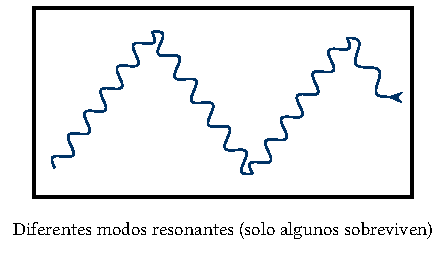
\includegraphics{figuras/cavidad-resonante.pdf}
\end{figure}
Sin entrar en mucho detalle, tenemos una cavidad de volumen $V$, cuyas paredes reflejan las ondas
electromagnéticas; las condiciones de frontera dadas por el contenedor permiten que solo ciertas
soluciones con ciertas frecuencias sean admisibles, llamados \textbf{modos resonantes}. Este tipo de
sistemas es llamado \textbf{cavidad resonante}.

Dentro de la cavidad la radiación se comporta como un gas de fotones, cuya energía está dada por la
ley de Stefan--Boltzmann:
\begin{equation*}
  \boxed{U=bVT^{4}}\qquad\text{con }b=7.56\times10^{-16}\ \mathrm{J/(m^{3}K^{4})}
\end{equation*}
(no confundir esta $b$ con la constante $b$ de van der Waals). La presión del gas de fotones
(presión de radiación) está dada por
\begin{equation*}
  \boxed{P=\frac{U}{3V}}
\end{equation*}
Ambas relaciones son de tipo empírico.

La radiación electromagnética no tiene partículas con masa (solo contiene fotones), por lo que $N$
no aparece en este tipo de sistemas y la relación fundamental es del tipo $S=S(U,V)$, por lo que, de
acuerdo con la ecuación de Euler,
\begin{equation*}
  S=\frac{1}{T}\,U+\frac{P}{T}\,V.
\end{equation*}
Reescribiendo las ecuaciones de estado de forma apropiada,
$\dfrac{1}{T^{4}}=\dfrac{bV}{U}$, o bien
\begin{equation*}
  \boxed{\frac{1}{T}=b^{1/4}\left(\frac{V}{U}\right)^{1/4}}
\end{equation*}
y multiplicando $\dfrac{1}{T}$ por $P$, se obtiene
\begin{equation*}
  P\,\frac{1}{T}=\frac{U}{3V}\,b^{1/4}\left(\frac{V}{U}\right)^{1/4}=\frac{1}{3}\,b^{1/4}\left(\frac{U}{V}\right)^{3/4}
  \quad\Longrightarrow\quad
  \boxed{\frac{P}{T}=\frac{1}{3}\,b^{1/4}\left(\frac{U}{V}\right)^{3/4}}
\end{equation*}
por lo cual la relación fundamental es
\begin{align*}
  S&=\left[b^{1/4}\left(\frac{V}{U}\right)^{1/4}\right]U+\left[\frac{1}{3}\,b^{1/4}\left(\frac{U}{V}\right)^{3/4}\right]V\\
   &=b^{1/4}V^{1/4}U^{3/4}+\frac{1}{3}\,b^{1/4}U^{3/4}V^{1/4}
   \quad\Longrightarrow\quad
   \boxed{S=\frac{4}{3}\,b^{1/4}V^{1/4}U^{3/4}}
\end{align*}

\subsection*{La banda elástica}

Considerando ahora un modelo donde se estudian las propiedades físicas de una banda elástica, capaz
de realizar trabajo
cuando se estira o se contrae. Este tipo de sistemas puede servir como un modelo de juguete para
describir otro tipo de sistemas físicos en donde las propiedades mecánicas de los medios continuos
(propiedades elásticas) son importantes.

La banda elástica está formada por un conjunto de moléculas de polímero en cadenas largas.
\begin{figure}[H]
  \centering
  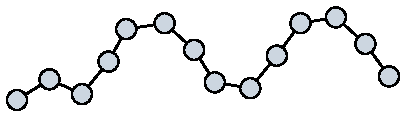
\includegraphics{figuras/polimero.pdf}
\end{figure}
Macroscópicamente, las cantidades de interés son las siguientes:
\begin{enumerate}[label=\arabic*.,itemsep=0pt]
  \item Longitud de la banda $L$ (equivale al volumen en los gases).
  \item Tensión $\mathcal{T}$ (análoga a la presión, pero negativa): $\mathcal{T}\sim-P$.
  \item Temperatura $T$.
  \item Energía interna.
\end{enumerate}
Se podría agregar un análogo al número de moles $N$, asociado con el número de unidades de monómeros
en la banda elástica; sin embargo, en general, este número no varía, por lo que se puede tener como
constante e ignorar del análisis.

Cualitativamente, se puede establecer que experimentalmente se observa que, si $L$ se mantiene
constante, $\mathcal{T}$ se incrementa con la temperatura $T$. Asimismo, dentro del llamado
\emph{límite elástico} (sin deformaciones permanentes al material), se observa que la energía es
\emph{independiente de la longitud de la banda}. La forma más simple para la energía de este sistema
es
\begin{equation*}
  \boxed{U=cL_0T}
\end{equation*}
con $c$ una constante y $L_0$ la longitud sin estirar la banda elástica.

Por otra parte, dentro del mismo régimen elástico también se observa que la tensión $\mathcal{T}$ es
linealmente proporcional a la elongación entre $L_0$ y $L_1$, siendo $L_1$ la longitud en la que la
banda alcanza el límite elástico, por lo que se tiene
\begin{equation*}
  \boxed{\mathcal{T}=bT\,\frac{L-L_0}{L_1-L_0}}\qquad\text{con }L_0\leq L<L_1,
\end{equation*}
donde $b$ es la constante de proporcionalidad para la longitud.
% NOTA: el manuscrito dice "la tensión entre L_0 y L_1"; por el contexto (y la fórmula) es la elongación (L-L_0)/(L_1-L_0).

En esta relación se incluye el factor $T$ (en lugar de $T^{2}$ o cualquier otra $f(T)$) para que esta
ecuación de estado sea consistente con el teorema de Schwarz, es decir,
\begin{equation*}
  \frac{\partial^{2}S}{\partial L\,\partial U}=\frac{\partial^{2}S}{\partial U\,\partial L}
  \qquad\text{o}\qquad
  \pdv{L}\left(\pdvc{S}{U}{L}\right)_{U}=\pdv{U}\left(\pdvc{S}{L}{U}\right)_{L},
\end{equation*}
con $\pdvc{S}{U}{L}=\dfrac{1}{T}$ y $\pdvc{S}{L}{U}=-\dfrac{\mathcal{T}}{T}$; por lo tanto
\begin{equation*}
  \left[\pdv{L}\left(\frac{1}{T}\right)\right]_{U}=\left[\pdv{U}\left(-\frac{\mathcal{T}}{T}\right)\right]_{L}.
\end{equation*}
De este modo, el factor lineal debe aparecer en la relación de $\mathcal{T}$ para que, al despejar,
quede proporcional a $1/T$ y del otro lado no aparezca $T$.

Entonces, las ecuaciones de estado son
\begin{equation*}
  U=cL_0T,\qquad\frac{1}{T}=\frac{cL_0}{U},\qquad
  \mathcal{T}=bT\,\frac{L-L_0}{L_1-L_0},\qquad-\frac{\mathcal{T}}{T}=-b\,\frac{L-L_0}{L_1-L_0}.
\end{equation*}
Si sustituimos en la relación para las variaciones de la entropía,
\begin{equation*}
  \dd S=\pdvc{S}{U}{L}\dd U+\pdvc{S}{L}{U}\dd L
  =\frac{1}{T}\,\dd U-\frac{\mathcal{T}}{T}\,\dd L
  =\frac{cL_0}{U}\,\dd U-b\,\frac{L-L_0}{L_1-L_0}\,\dd L,
\end{equation*}
e integrando,
\begin{equation*}
  \boxed{S=S_0+cL_0\ln\frac{U}{U_0}-\frac{b}{2(L_1-L_0)}\,(L-L_0)^{2}}
\end{equation*}
A pesar de que esta relación se construyó a partir de información cualitativa, representa de forma
empírica las propiedades de este tipo de sistemas de forma consistente.

\section{Energía interna. Entropía. Postulado de máxima entropía}

\subsection*{Energía interna}

El descubrimiento del principio de conservación de la energía en física representó un avance muy
importante.

Leibniz (1693) fue el primero en notar que
\begin{equation*}
  \tfrac{1}{2}mv^{2}+mgh=\text{cte. de movimiento}
\end{equation*}
para una masa puntual moviéndose en el campo gravitacional terrestre, donde $\vec{F}=-\nabla\Phi$.
% NOTA (manuscrito): al margen aparece $\frac{D\phi}{Dt}=\frac{\partial\phi}{\partial t}+\vec{u}\cdot\nabla\phi$ con una flecha hacia $\vec{F}=-\nabla\Phi$.
Esto puede extenderse a otro tipo de sistemas, como los sistemas electrostáticos, a los sistemas
relativistas (Einstein) o nucleares (Fermi?).

Desde un punto de vista moderno, los principios de conservación se entienden como una consecuencia
del hecho de que las leyes de la física son las mismas desde hace mucho tiempo y así seguirán, es
decir, son invariantes ante $t\to t+t'$ con $t'$ una constante (un corrimiento temporal). Así,
el principio de conservación de la energía es uno de los principios más fundamentales,
significativos y generales de todas las teorías físicas. En el caso de los sistemas
termodinámicos veamos su importancia.

Para un sistema macroscópico formado por un gran número de partículas, en donde existen
interacciones (fuerzas) que pueden ser complicadas pero que al mismo tiempo están bien definidas y
para las cuales también se aplican principios de conservación, se puede concluir entonces que,
desde el punto de vista macroscópico, \emph{los sistemas macroscópicos tienen energías bien
definidas, y están sujetas a un principio de conservación bien definido}.

\begin{postulado}[Energía interna]
  Se asume que un sistema termodinámico tiene una energía bien definida, la cual es una
  manifestación de un principio o ley de conservación (primera ley de la termodinámica).
\end{postulado}

Históricamente, la existencia de una función termodinámica para la energía fue demostrada por
medios puramente macroscópicos, ya que durante finales del siglo XVIII y hasta mediados del siglo
XIX no se conocía la existencia de las partículas microscópicas (Carnot, Davy, Mayer, Joule y
Rumford).

Asimismo, heredado de la mecánica newtoniana, no debemos olvidar que en el caso de la energía solo
las \emph{diferencias} de energía son importantes, no los valores absolutos de esta.
\begin{observacion}
  Los valores de energía son siempre relativos y no hay un valor mínimo universal: se puede fijar
  arbitrariamente. Lo importante es siempre cómo cambia la energía entre dos estados.
\end{observacion}

\begin{definicion}[Energía interna]
  La función termodinámica de la energía del sistema macroscópico es llamada \textbf{energía
  interna}, $U$; es un reflejo de la conservación de la energía de los elementos microscópicos como
  un todo.
\end{definicion}

Un sistema macro multicomponente queda descrito por $(U,V,N_1,N_2,\dots,N_K)$. Si se unen dos
sistemas idénticos $(U,V,N)$ se obtiene
\begin{equation*}
  (U,V,N)+(U,V,N)=(2U,2V,2N),
\end{equation*}
\begin{figure}[H]
  \centering
  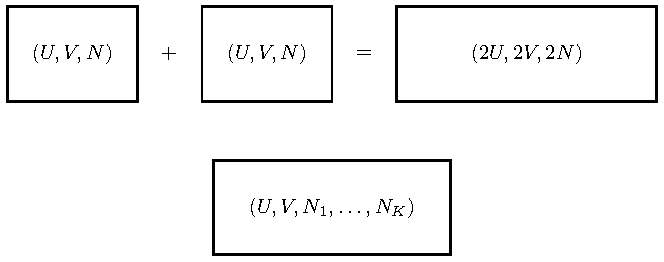
\includegraphics{figuras/extensivos-U.pdf}
\end{figure}
es decir, la energía interna $U$ también es una cantidad extensiva.

\begin{definicion}[Variables extensivas]
  Las variables termodinámicas cuyo valor depende del tamaño del sistema son llamadas
  \textbf{variables extensivas} del sistema.
\end{definicion}

Por lo tanto, el conjunto de variables (coordenadas) $(U,V,N)$ es un conjunto de variables
termodinámicas extensivas.

\subsection*{El problema central de la termodinámica}

El problema central que define la termodinámica es el siguiente:

\begin{quote}
  <<Determinar el estado de equilibrio que eventualmente resulta después de remover restricciones
  internas en un sistema compuesto y cerrado.>>
\end{quote}

\begin{figure}[H]
  \centering
  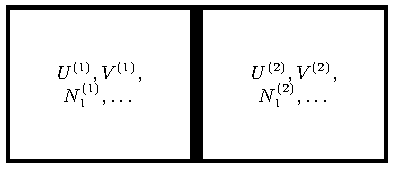
\includegraphics{figuras/cilindro-compuesto.pdf}
\end{figure}
Supongamos que dos sistemas simples están contenidos dentro de un cilindro, separados el uno del
otro por un pistón interno. Se asume que las paredes del cilindro y el pistón son rígidos,
impermeables a la materia, adiabáticos, y que la posición del cilindro está firmemente fija;
asimismo, cada sistema es cerrado.
\begin{itemize}[itemsep=2pt]
  \item Si se libera el pistón (es decir, se remueve una de las restricciones del sistema), este
    buscará en general una nueva posición (ya que está atravesando un proceso de cambio de
    volumen).
  \item Por otro lado, si se le remueve la cobertura adiabática al pistón fijo (es decir, se
    remueve otra restricción), de manera que el calor pueda fluir libremente entre los dos
    sistemas, entonces habrá una redistribución de la energía térmica entre ambos sistemas.
  \item Si se perfora el pistón (otra restricción se remueve), habrá una redistribución de la
    materia (y de la energía).
\end{itemize}
La remoción de una restricción, en cada caso, resulta en el inicio de un \textbf{proceso
espontáneo}, y cuando finalmente el sistema se establece en nuevos estados de equilibrio, se tienen
nuevos valores de los parámetros $U^{(1)},V^{(1)},N_1^{(1)},\dots$ y $U^{(2)},V^{(2)},N_1^{(2)},\dots$
El problema central de la termodinámica es el cálculo de los valores de equilibrio de esos
parámetros.

\begin{definicion}[Restricción interna]
  Cualquier construcción (restricción) que evite el flujo de energía, materia o el cambio de
  volumen entre sistemas simples que están en contacto entre sí (sistema compuesto) y cerrados con
  el resto del universo es llamada \textbf{restricción interna}.
\end{definicion}

Si un sistema termodinámico compuesto está en equilibrio con respecto a un conjunto de
restricciones internas y algunas de estas son removidas, ciertos procesos que no eran accesibles se
vuelven posibles. Estos procesos llevan al sistema a un estado de equilibrio. Este es el problema
central de la termodinámica.

\subsection*{Entropía y principio de máxima entropía}

Históricamente, la formulación del principio que tuvo por objetivo resolver el problema central de
la termodinámica fue un proceso complejo, por lo que es más conveniente presentarlo de forma
natural como una serie de postulados que dependen de una justificación \emph{a posteriori} (en
lugar de \emph{a priori}).

Partamos de la pregunta: ¿cuál es el criterio más simple que se puede considerar (y que sea
razonable) para determinar los estados de equilibrio finales que se alcanzan después de quitar una
restricción interna?

A partir de lo que sabemos de física (mecánica) podríamos esperar que la forma más económica en la
que un sistema alcanza un estado de equilibrio es cuando un parámetro de estos sistemas se
\emph{extremiza} (en mecánica, en general, la energía es un mínimo; por ejemplo, una partícula en
un pozo de potencial cae hacia el mínimo).
\begin{figure}[H]
  \centering
  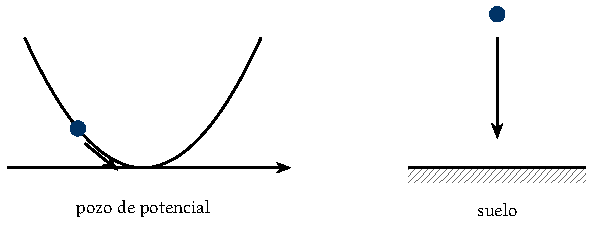
\includegraphics{figuras/pozo-potencial.pdf}
\end{figure}

Por lo tanto, en termodinámica es sensato pensar que un estado de equilibrio termodinámico se
alcanzará cuando los valores que toman los parámetros extensivos en algún estado de equilibrio
final sean tales que extremicen (ya sea maximicen o minimicen) alguna función.
\begin{observacion}
  Maximizar o minimizar son equivalentes, ya que dependen únicamente de una convención de signos,
  pero no afectan la estructura lógica de la teoría.
\end{observacion}
Sería deseable que esta función hipotética tuviese otras propiedades matemáticas deseables, en
particular que sea suficientemente simple para garantizar que la teoría que se derive de ella sea
lo suficientemente simple. Se desarrolla esta solución propuesta en una serie de postulados.

\begin{postulado}[II: principio de máxima entropía]
  Existe una función (llamada \textbf{entropía} $S$) de los parámetros extensivos de un sistema
  compuesto, definida para todos los estados de equilibrio y que tiene la siguiente propiedad: los
  valores asumidos por los parámetros extensivos en ausencia de restricciones internas son tales que
  \textbf{maximizan la entropía sobre la variedad de estados de equilibrio}.
\end{postulado}

\begin{definicion}[Variedad]
  Una \textbf{variedad} $n$-dimensional es un conjunto que, alrededor de cada uno de sus puntos, se
  comporta como un espacio euclidiano $\R^n$: cada punto de la variedad tiene una vecindad que puede
  ser mapeada de forma continua y reversible a un subconjunto abierto de $\R^n$.
\end{definicion}
% NOTA (manuscrito): al margen se listan los tipos de variedad: topológica, diferencial, riemanniana, algebraica.

En el postulado II solo se establece la existencia de $S$ para estados de equilibrio, y este mismo no
hace referencia a estados de no equilibrio. Además, en ausencia de alguna restricción, el sistema es
libre de acceder a alguno de un número de estados, cada uno de los cuales puede ser accesible en
presencia de alguna restricción adecuada. La entropía de cada uno de estos estados de equilibrio
constreñido está definida, y la entropía toma el valor más grande para alguno de esos estados en
particular. En ausencia de la restricción, este estado de máxima entropía es aquel seleccionado por
el sistema.

\begin{ejemplo}
  Sean dos sistemas, $(1)$ y $(2)$, separados por una pared diatérmica (intercambio de calor), que
  forman un sistema compuesto con parámetros $U^{(1)},V^{(1)},N^{(1)}$ y $U^{(2)},V^{(2)},N^{(2)}$.
  \begin{figure}[H]
    \centering
    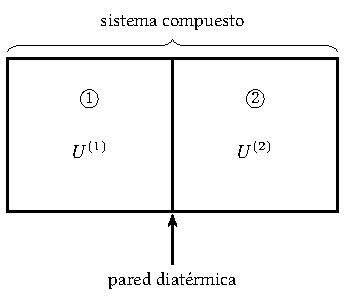
\includegraphics{figuras/sistema-compuesto.pdf}
  \end{figure}
  ¿Cómo se distribuye la energía interna total $U$ entre los dos sistemas? Se tiene
  \begin{equation*}
    U=U^{(1)}+U^{(2)},\qquad\text{sujeto a lo siguiente:}
  \end{equation*}
  para cada estado de equilibrio constreñido del sistema existe una entropía para el sistema
  compuesto y, para algunos valores particulares de $U^{(1)}$ y $U^{(2)}$, esta entropía es un
  máximo. Estos son entonces los valores de $U^{(1)}$ y $U^{(2)}$ que se obtienen en presencia de
  una pared diatérmica o en ausencia de una constricción adiabática.
\end{ejemplo}

\section{Temperatura y equilibrio térmico (ley cero)}

\subsection*{Equilibrio térmico y la ley cero de la termodinámica}

Los sistemas macroscópicos usualmente exhiben ``memoria'' de su evolución reciente (estos
fenómenos se relacionan con efectos como la inercia, los transcientes, turbulencias). Por ejemplo:
\begin{itemize}[itemsep=0pt]
  \item osciladores forzados,
  \item movimiento de fluidos,
  \item esfuerzos elásticos,
  \item mezclas.
\end{itemize}
Eventualmente, este tipo de fenómenos desaparece, en algunos casos de forma muy rápida (pocos
segundos) o muy lenta (hasta decenas de años), regresando los sistemas a estados físicos más
simples, los cuales son independientes de la historia de estos.

\begin{definicion}[Estado físico]
  Situación o forma en la que se encuentra un sistema físico, caracterizado por un conjunto de
  variables que lo describen. Dos estados son iguales si y solo si las variables que los
  caracterizan son idénticas.
\end{definicion}

En la naturaleza los sistemas tienden a evolucionar hacia estados en los que no cambian, a menos
que fuerzas externas actúen sobre ellos. A partir de este hecho podemos establecer que
\emph{todos los sistemas tienden a evolucionar hacia estados en los cuales las propiedades que los
describen son determinadas por factores intrínsecos (que se asocian al sistema mismo) y no por
influencias externas a estos.} Tales estados simples son, por definición, independientes del
tiempo. Este tipo de estados son llamados \textbf{estados de equilibrio}.

\begin{ejemplo}
  Una taza de café siendo agitada (no es un estado de equilibrio).
\end{ejemplo}

La termodinámica busca entonces describir estos estados estáticos de equilibrio hacia los cuales
los sistemas eventualmente evolucionan.

Expresar este objetivo desde un punto de vista formal no es trivial y existen diversas formas de
lograrlo. La forma más usual es a través de la llamada \textbf{ley cero de la termodinámica}, para
lo cual es necesario dar una definición del concepto de temperatura y los procesos irreversibles.
En este caso vamos a saltar por un momento esta definición y daremos una definición equivalente.

\begin{postulado}[I: estados de equilibrio]
  Existe un conjunto de estados particulares (llamados \emph{estados de equilibrio}) de los
  sistemas simples, los cuales están completamente caracterizados por la energía interna $U$, el
  volumen $V$ y el número de moles $N_1,N_2,\dots,N_K$ de los componentes químicos.
\end{postulado}

Este postulado se puede generalizar para incluir otras propiedades.

Aquellos sistemas que no se encuentran en estados de equilibrio no pueden ser analizados por la
termodinámica tal como la hemos planteado (usualmente llamada \textbf{termodinámica de
equilibrio}), ya que resultaría en discrepancias en la información obtenida.

Desde el punto de vista micro, los sistemas pasan a través de un gran número de cambios en las
partículas que los forman (transiciones atómicas, ionizaciones, colisiones, etc.) pero que tienen
poco o nulo efecto macro. En realidad, desde el punto de vista micro los sistemas termodinámicos
no están en equilibrio, pero desde el punto de vista macro los sistemas prácticamente están en
equilibrio.

Asimismo, por otro lado existen procesos macroscópicos tan lentos (por ejemplo, decaimientos
radiactivos) que tardan escalas cósmicas en ocurrir (evaporación de agujeros negros), que se puede
asumir que están prácticamente en un estado de equilibrio. Podemos decir entonces que,
\emph{operacionalmente}, un sistema se encuentra en un estado de equilibrio si sus propiedades son
descritas consistentemente por la termodinámica de equilibrio.

Regresando a la ley cero de la termodinámica (Ralph Fowler, 1930), partamos de la siguiente
situación: sean dos o más sistemas termodinámicos en contacto entre sí que interactúan
intercambiando energía/materia.
\begin{figure}[H]
  \centering
  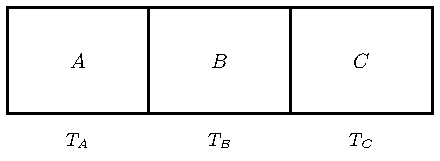
\includegraphics{figuras/ley-cero.pdf}
\end{figure}

\begin{ley}[Ley cero de la termodinámica]
  Existe una cantidad termodinámica llamada \textbf{temperatura} (no daremos más detalles por el
  momento) tal que, eventualmente, será igual entre sistemas en contacto solo cuando se alcance un
  estado de equilibrio llamado \textbf{equilibrio térmico}:
  \begin{equation*}
    T_A=T_B\iff A\text{ está en equilibrio térmico con }B.
  \end{equation*}
  Además, si el sistema $A$ está en equilibrio térmico con $B$ y $B$ está en equilibrio con $C$,
  entonces $A$ está en equilibrio con $C$:
  \begin{equation*}
    T_A=T_B\ \text{ y }\ T_B=T_C\ \Longrightarrow\ T_A=T_C.
  \end{equation*}
\end{ley}

Es decir, la temperatura es una propiedad \emph{transitiva}: una propiedad que puede compararse
entre sistemas que no interactúan directamente.
% NOTA: en el manuscrito la última implicación está escrita con "$\Longleftrightarrow$"; se corrigió a "$\Longrightarrow$".

\subsection*{Temperatura e isotermas}

Sobre la temperatura:
\begin{align*}
  \text{Temperatura}&\xrightarrow{\text{def.\ empírica}}\text{sensación de calor o frío},\\
  \text{Temperatura}&\xrightarrow{\text{def.\ termodinámica}}\text{equilibrio térmico: }T_A=T_B,
\end{align*}
donde la temperatura es la cantidad que es igual entre dos sistemas cuando se alcanza este estado.

Supongamos que un cierto sistema $A$ está descrito por dos variables termodinámicas $X$ y $Y$, y
otro sistema $B$ está descrito por dos variables termodinámicas $X'$ y $Y'$. Si $A$ está en un
estado descrito por $(X_1,Y_1)$ y además está en equilibrio térmico con $B$, cuyo estado está
descrito por $(X_1',Y_1')$, y el estado del sistema $A$ cambia a otro descrito por $(X_2,Y_2)$,
eventualmente el sistema $B$ alcanzará un estado de equilibrio térmico descrito por
$(X_2',Y_2')$ (donde $X_1\neq X_2$, $Y_1\neq Y_2$, $X_1'\neq X_2'$ y $Y_1'\neq Y_2'$ en general).
Este proceso puede repetirse muchas veces (en principio, un número infinito).

Si quisiéramos estudiar la evolución de los estados de equilibrio térmico de los sistemas $A$ y
$B$, es posible hacerlo de un modo geométrico a través de las variables $(X,Y)$ y $(X',Y')$ en
un diagrama $X$--$Y$ (sistema $A$) y un diagrama $X'$--$Y'$ (sistema $B$).
\begin{figure}[H]
  \centering
  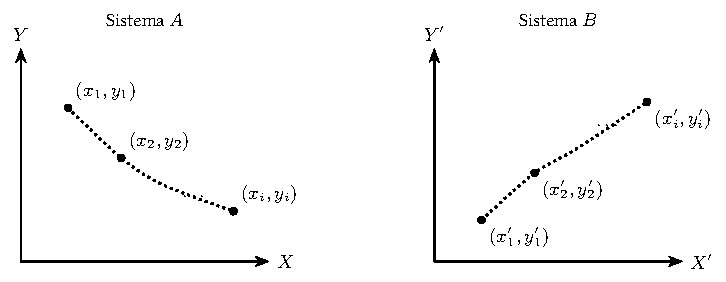
\includegraphics{figuras/isotermas.pdf}
\end{figure}
Se puede construir una curva para cada sistema atravesando cada uno de estos estados de equilibrio
térmico. Podemos asumir que todos estos estados, donde $T_1=T_1',\,T_2=T_2',\,\dots,\,T_n=T_n'$
(para $n$ estados de equilibrio térmico), yacen en una curva llamada \textbf{isoterma}
(temperaturas iguales).

\begin{definicion}[Isoterma]
  Una isoterma es el lugar geométrico de todos los puntos que representan estados en los que un
  sistema está en equilibrio térmico con un estado de otro sistema.
\end{definicion}

\subsection*{Equilibrio térmico y temperatura}

Ahora estudiaremos algunas de las consecuencias del principio extremal postulado para la entropía.
Sea un sistema cerrado compuesto por dos sistemas simples separados por una pared impermeable al
flujo de
materia (partículas), pero que permite el intercambio de calor.
\begin{figure}[H]
  \centering
  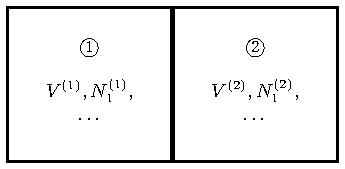
\includegraphics{figuras/pared-impermeable.pdf}
\end{figure}
Entonces el volumen y el número de moles \emph{están fijos}, pero $U^{(1)}$ y $U^{(2)}$ pueden
cambiar, aunque están sujetos a la restricción
\begin{equation*}
  U^{(1)}+U^{(2)}=\text{cte.},
\end{equation*}
ya que el sistema es un sistema cerrado.

Asumiendo que el sistema alcanza el equilibrio, de acuerdo con el postulado II debemos buscar
aquellos valores de los parámetros extensivos tales que maximizan el valor que toma $S$ sobre la
variedad de estados de equilibrio. Para hallar este extremo, uno de los requerimientos matemáticos
de este caso particular es que, una vez que se alcanza el estado de equilibrio, una transferencia
infinitesimal \emph{virtual} (ya que es una transferencia hipotética de energía, para analizar el
comportamiento del sistema) de energía del sistema $1$ al $2$ no producirá cambios en la entropía:
\begin{equation*}
  \dd S=0\qquad(\text{implica que }S\text{ es un extremo}).
\end{equation*}
Además, de acuerdo con el postulado III, la entropía es una función aditiva sobre los sistemas
constituyentes. Por lo tanto,
\begin{equation*}
  S=S^{(1)}\bigl(U^{(1)},V^{(1)},N_1^{(1)},\dots,N_j^{(1)},\dots\bigr)+S^{(2)}\bigl(U^{(2)},V^{(2)},N_1^{(2)},\dots,N_j^{(2)},\dots\bigr).
\end{equation*}
Debido a la transferencia virtual de energía de $1$ a $2$, el cambio de la entropía es entonces
\begin{equation*}
  \dd S=\pdvc{S^{(1)}}{U^{(1)}}{V^{(1)},\dots,N_j^{(1)},\dots}\dd U^{(1)}+\pdvc{S^{(2)}}{U^{(2)}}{V^{(2)},\dots,N_j^{(2)},\dots}\dd U^{(2)},
\end{equation*}
y con la definición de los parámetros intensivos entrópicos,
\begin{equation*}
  \dd S=\frac{1}{T^{(1)}}\dd U^{(1)}+\frac{1}{T^{(2)}}\dd U^{(2)};
\end{equation*}
además, de acuerdo con el principio de máxima entropía,
\begin{equation*}
  \dd S=0=\frac{1}{T^{(1)}}\dd U^{(1)}+\frac{1}{T^{(2)}}\dd U^{(2)}.
\end{equation*}
Asimismo, de acuerdo con la conservación de la energía, $U^{(1)}+U^{(2)}=\text{cte.}$; diferenciando,
$\dd U^{(1)}+\dd U^{(2)}=0$, es decir, $\dd U^{(1)}=-\dd U^{(2)}$. Sustituyendo $\dd U^{(2)}$,
\begin{equation*}
  \frac{1}{T^{(1)}}\dd U^{(1)}-\frac{1}{T^{(2)}}\dd U^{(1)}=0
  \qquad\text{o bien}\qquad
  \left(\frac{1}{T^{(1)}}-\frac{1}{T^{(2)}}\right)\dd U^{(1)}=0.
\end{equation*}
Ya que el caso trivial es que $\dd U^{(1)}=0$ (no habrá transferencia de energía), se concluye
\begin{equation*}
  \boxed{\frac{1}{T^{(1)}}-\frac{1}{T^{(2)}}=0}\quad\text{(rep.\ entrópica)}
  \qquad\text{o}\qquad
  \boxed{T^{(1)}=T^{(2)}}\quad\text{(rep.\ energética)}.
\end{equation*}
Esto es llamado \textbf{condición de equilibrio térmico}.

Este problema puede seguirse estudiando al analizar las condiciones de estabilidad, cuando además de
cumplir que $\dd S=0$ (extremo) se debe satisfacer que $\dd^{2}S<0$ (máximo).

\subsubsection*{Relación del equilibrio térmico con el concepto intuitivo de $T$}

Del caso anterior, si dos sistemas están separados por una pared diatérmica, el calor fluirá hasta
que el sistema compuesto tenga la misma temperatura; lo anterior está de acuerdo con la noción
intuitiva de la temperatura. Para ahondar con mayor detalle en esto, se puede estudiar el caso
anterior con mayor detalle.
\begin{figure}[H]
  \centering
  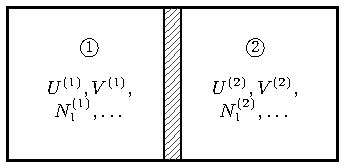
\includegraphics{figuras/pared-adiabatica.pdf}
\end{figure}
Asumiendo que la pared que separa a los sistemas $1$ y $2$ es adiabática y que la temperatura de los
dos sistemas es muy semejante, pero no exactamente igual, en particular se asume que:
\begin{equation*}
  T^{(1)}>T^{(2)}.
\end{equation*}
Se considera que el sistema está inicialmente en equilibrio con respecto a la constricción
adiabática interna. Si se remueve la constricción, el sistema ya no se encuentra en equilibrio y el
calor fluye a través de la pared; por lo que la entropía del sistema compuesto se incrementa.
Finalmente, el sistema alcanza un nuevo estado de equilibrio, determinado por la condición de que
$T^{(1)}=T^{(2)}$, y el máximo valor de $S$ posible se alcanza. Sea $\Delta S$ la diferencia de
entropías entre el estado final e inicial; se cumple que
\begin{equation*}
  \Delta S>0.
\end{equation*}
Por lo que, de acuerdo con la variación de $S$ y la conservación de la energía,
$\dd S=\left(\frac{1}{T^{(1)}}-\frac{1}{T^{(2)}}\right)\dd U^{(1)}$, y por tanto
\begin{equation*}
  \Delta S\simeq\left(\frac{1}{T^{(1)}}-\frac{1}{T^{(2)}}\right)\Delta U^{(1)},
\end{equation*}
donde $T^{(1)}$ y $T^{(2)}$ son los valores iniciales de las temperaturas. Pero como
$T^{(1)}>T^{(2)}$ (es decir, $\frac{1}{T^{(1)}}<\frac{1}{T^{(2)}}$), se sigue que, para que
$\Delta S>0$,
\begin{equation*}
  \Delta U^{(1)}<0.
\end{equation*}
Por lo que se concluye que el calor ha fluido desde el subsistema $1$ hacia el subsistema $2$. De
manera que el calor tiende a fluir desde un sistema con una temperatura alta hacia uno con una
temperatura más baja. Esto está en concordancia con la noción intuitiva de $T$. Además, esta
conclusión no depende de la suposición de que $T^{(1)}$ es aproximadamente igual a $T^{(2)}$.

Nuestra noción intuitiva de temperatura, basada en la sensación psicológica de frío y calor, se
basa en dos propiedades: $T$ es un parámetro intensivo (porque tiene el mismo valor en una parte
del sistema que en todo el mismo) y, en segundo lugar, el calor fluye desde regiones de alta
temperatura hacia regiones de baja temperatura. Por lo que el equilibrio térmico se asocia con la
igualdad y homogeneidad de la temperatura.

\subsubsection*{Unidades de temperatura}

Como $T\equiv\pdv{U}{S}$, las dimensiones de $T$ deben ser entonces $[T]=\left[\dfrac{U}{S}\right]$;
para determinar las dimensiones de $T$, se deben determinar las dimensiones de $S$. Si se multiplica
$S$ por una constante dimensional positiva, se obtiene una nueva función de dimensiones diferentes,
pero que tiene exactamente las mismas propiedades extremales, por lo que también es una elección
aceptable para la entropía. Podemos decir que $S$ es una cantidad adimensional; por lo tanto, las
dimensiones de $T$ deben ser dimensiones de energía:
\begin{equation*}
  S\propto\ln\Omega\qquad\text{y}\qquad S=k_B\ln\Omega,
\end{equation*}
donde $\Omega$ es un número (el número de microestados accesibles) y $k_B$ es la constante de
proporcionalidad.
% NOTA: en el manuscrito solo se rotula "número" sobre Ω y "cte. de proporcionalidad" sobre k_B; la interpretación de Ω como número de microestados es la usual (se verá en mecánica estadística).

Sin embargo, como sucede en otros casos [e.g., trabajo (J) y torque (N$\cdot$m) tienen la misma
dimensión pero diferentes unidades], en física diferentes tipos de cantidades físicas deben tener
diferentes unidades, con el mismo tipo de dimensiones. Entonces
\begin{equation*}
  [T]=\frac{M\,L^{2}}{t^{2}}=[U],
\end{equation*}
donde $t$ denota tiempo; para $U$ las unidades son J, erg, cal, etc.

Más adelante veremos que los principios de la termodinámica nos dan un procedimiento experimental
que determina sin ambigüedad la razón de las temperaturas de cualesquiera dos sistemas dados
(eficiencia y motores de Carnot).
\begin{figure}[H]
  \centering
  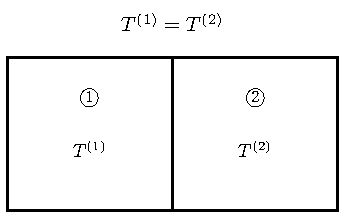
\includegraphics{figuras/temperaturas-iguales.pdf}
\end{figure}
El hecho de poder medir la razón de temperaturas tiene dos consecuencias importantes:
\begin{enumerate}[label=\arabic*.,itemsep=2pt]
  \item La temperatura está determinada unívocamente y no puede ser arbitrariamente asignada o
    ``trasladada'' (multiplicada por una constante).
  \item Somos libres de asignar el valor de unidad (u otro valor) a un estado arbitrario, con lo que
    se pueden asignar los valores de cualquier otro estado.
\end{enumerate}
Equivalentemente, el único aspecto arbitrario de las escalas de temperatura es el tamaño de la
unidad de temperatura, la cual se determina al asignar una temperatura específica a algún estado
particular de un sistema estandarizado.

\subsubsection*{Escalas de temperatura}

Las escalas de temperatura surgen al asignar diferentes valores de $T$ a estados estandarizados,
pero todas las escalas deben coincidir en $T=0$. Además, de acuerdo con el postulado de
Planck--Nernst, $T$ siempre es una cantidad definida positiva.
% NOTA: el manuscrito dice "teorema de Planck-Nernst"; en las páginas anteriores se le llama postulado (IV).

\begin{definicion}[Escala Kelvin]
  La escala Kelvin de temperatura (la cual es la escala de $T$ en el SI de medidas) se define al
  asignar el número $273.16$ a la temperatura de una mezcla de hielo puro, agua y vapor en equilibrio
  mutuo (\emph{punto triple del agua}), el cual determina una temperatura única. La unidad de esta
  escala es el kelvin (K).
\end{definicion}

La razón entre las unidades kelvin y joule (recordando que son dimensionalmente iguales) es
$1.3806\times10^{-23}\ \mathrm{J/K}$; esta razón es usualmente llamada \textbf{constante de
Boltzmann} ($k_B$), por lo que la cantidad $k_BT$ tiene dimensiones de energía:
\begin{equation*}
  k_B=1.3806\times10^{-23}\ \mathrm{J/K}.
\end{equation*}

\begin{definicion}[Escala Rankine]
  La escala Rankine se obtiene al asignar la temperatura
  $\left(\tfrac{9}{5}\right)(273.16)=491.688\ ^{\circ}\mathrm{R}$ al punto triple del agua. La unidad
  es llamada grado Rankine ($^{\circ}\mathrm{R}$) y la temperatura Rankine es simplemente $9/5$ la
  temperatura Kelvin.
\end{definicion}

También se puede definir una escala relacionada con la Kelvin llamada \textbf{escala Kelvin
internacional}, definida en términos de las propiedades de sistemas particulares en diferentes
rangos de temperatura, escogidos tan cerca como es posible a la escala Kelvin absoluta. Esta escala
permite tener estándares para la medición de temperatura en el laboratorio. Sin embargo, esta no es
una escala termodinámica verdadera (no coincide con $T=0$ con lo establecido en el postulado IV).

En las escalas K y $^{\circ}\mathrm{R}$ los rangos usuales de sistemas cercanos a la temperatura
ambiente son de $300\ \mathrm{K}$ y $540\ ^{\circ}\mathrm{R}$.

\begin{definicion}[Escala Celsius]
  La escala Celsius se define como
  \begin{equation*}
    T(^{\circ}\mathrm{C})=T(\mathrm{K})-273.15,
  \end{equation*}
  donde $T(^{\circ}\mathrm{C})$ denota la temperatura Celsius, cuya unidad es denotada por
  $^{\circ}\mathrm{C}$. Esta escala se define en base a los siguientes estados estandarizados del agua:
  \begin{enumerate}[label=\arabic*.,itemsep=0pt]
    \item $0\ ^{\circ}\mathrm{C}$ corresponde a la temperatura de fusión del hielo (punto de
      congelación) a $1$ atm de presión.
    \item $100\ ^{\circ}\mathrm{C}$ corresponde a la temperatura de ebullición del agua a $1$ atm de
      presión.
  \end{enumerate}
  Entre estos dos estados se dividen $100$ intervalos iguales, que corresponden a
  $1\ ^{\circ}\mathrm{C}$.
\end{definicion}

(No comienza en el cero absoluto.) Dado que el cero en esta escala está desplazado respecto al cero
absoluto, esta escala no es una escala termodinámica real.
% VERIFICAR: el manuscrito dice "desplazado al punto triple de la mezcla de agua"; el cero Celsius (273.15 K) no es exactamente el punto triple (273.16 K).

\begin{definicion}[Escala Fahrenheit]
  La escala Fahrenheit de temperatura se define como
  \begin{equation*}
    T(^{\circ}\mathrm{F})\equiv T(^{\circ}\mathrm{R})-459.67=\frac{9}{5}\,T(^{\circ}\mathrm{C})+32.
  \end{equation*}
\end{definicion}

Para esta escala, la temperatura del punto de fusión del hielo a $1$ atm es de alrededor de
$32\ ^{\circ}\mathrm{F}$, y para el punto de ebullición del agua a $1$ atm es de alrededor de
$212\ ^{\circ}\mathrm{F}$. La temperatura ambiente está en la vecindad de $70\ ^{\circ}\mathrm{F}$.
El $0\ ^{\circ}\mathrm{F}$ se encuentra en el estado en el punto en el que el hielo, la sal y el
agua se encuentran en equilibrio.

Aunque nosotros hemos definido a la temperatura como $T\equiv\pdvc{U}{S}{X_i}$ de manera formal,
también es posible definirla en términos más convencionales siguiendo el método de
\textbf{Kelvin y Carathéodory}, que modela el espacio de estados de equilibrio como una variedad
diferenciable de dimensión $n+1$; en él, $\dbar Q=T\,\dd S$ define una distribución de hiperplanos
en la variedad.

El \textbf{teorema de Carathéodory} garantiza que, si en cada vecindad hay estados inaccesibles
adiabáticamente, entonces existe una función $S$ tal que $\dbar Q=T\,\dd S$. Con lo anterior, la
termodinámica se convierte en una teoría de \emph{variedades de contacto} (de dimensión impar).

El flujo de calor $\dbar Q$ se define a través del principio de conservación de la energía (tal y
como hicimos nosotros). A partir de ciertos procesos cíclicos, se infiere que existe un
\textbf{factor integrante} (es decir, el factor utilizado para convertir un diferencial inexacto en
un diferencial exacto) $1/T$, tal que el producto de dicho factor con el diferencial imperfecto
$\dbar Q$ da como resultado un diferencial perfecto:
\begin{equation*}
  \dd S=\frac{1}{T}\,\dbar Q\qquad(\text{diferencial de primer orden}).
\end{equation*}
De esta forma, la entropía y la temperatura se introducen como resultado del análisis de la
existencia de factores integrantes para un tipo de ecuaciones diferenciales (1-formas) llamadas
\textbf{formas pfaffianas}.

\begin{definicion}[1-forma diferencial]
  Una $1$-forma diferencial en una variedad diferencial es una expresión
  $\omega=\sum_{i=1}^{n}a_i(x_1,\dots,x_n)\,\dd x_i$, donde $a_i$ son funciones suaves y $\dd x_i$
  son diferenciales de las coordenadas. Se estudia su integrabilidad.
\end{definicion}

\section{Equilibrio mecánico y químico}

\subsection*{Equilibrio mecánico}

Similarmente al caso del equilibrio térmico, se puede llevar a cabo un proceso similar al
considerar un sistema cerrado compuesto por dos sistemas simples separados por una \emph{pared
diatérmica móvil} que no permite el flujo de materia.
\begin{figure}[H]
  \centering
  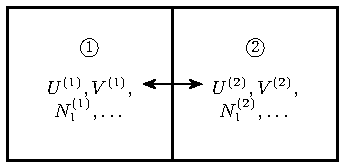
\includegraphics{figuras/pared-diatermica-movil.pdf}
\end{figure}
Los valores de los números de moles están fijos y son constantes. Además, los valores de $U^{(1)}$ y
$U^{(2)}$ pueden cambiar, pero están sujetos a la condición de cerradura dada por el principio de
conservación,
\begin{equation*}
  U^{(1)}+U^{(2)}=\text{cte.},
\end{equation*}
(condición necesaria para que el problema pueda ser resuelto: el problema está cerrado o aislado
dentro del sistema). Asimismo, los valores de $V^{(1)}$ y $V^{(2)}$ pueden cambiar, pero también
están sujetos a una condición de cerradura dada por el hecho de que el sistema está cerrado:
\begin{equation*}
  V^{(1)}+V^{(2)}=\text{cte.}
\end{equation*}

De nueva cuenta, el postulado II requiere que no existan cambios en la entropía como resultado de
procesos infinitesimales virtuales, los cuales consisten de transferencias de calor a través de la
pared o de desplazamientos de la pared. Entonces $\dd S=0$, y dado que
\begin{multline*}
  \dd S=\pdvc{S}{U^{(1)}}{V^{(1)},N_1^{(1)},\dots}\dd U^{(1)}+\pdvc{S}{V^{(1)}}{U^{(1)},N_1^{(1)},\dots}\dd V^{(1)}\\
  +\pdvc{S}{U^{(2)}}{V^{(2)},N_1^{(2)},\dots}\dd U^{(2)}+\pdvc{S}{V^{(2)}}{U^{(2)},N_1^{(2)},\dots}\dd V^{(2)}.
\end{multline*}
% NOTA: en el manuscrito el último término aparece con "dV^{(1)}"; por el contexto es dV^{(2)}.
Por las condiciones de cerradura podemos ver que los cambios en energía interna y en el volumen
resultan en
\begin{align*}
  \dd U^{(1)}+\dd U^{(2)}&=0\quad\text{o}\quad\dd U^{(2)}=-\dd U^{(1)},\\
  \dd V^{(1)}+\dd V^{(2)}&=0\quad\text{o}\quad\dd V^{(2)}=-\dd V^{(1)}.
\end{align*}
% NOTA: en el manuscrito la segunda igualdad se escribe "dV^{(2)}=-dV^{(2)}"; por el contexto es -dV^{(1)}.
Entonces,
\begin{equation*}
  \dd S=\left(\frac{1}{T^{(1)}}-\frac{1}{T^{(2)}}\right)\dd U^{(1)}+\left(\frac{P^{(1)}}{T^{(1)}}-\frac{P^{(2)}}{T^{(2)}}\right)\dd V^{(1)}=0.
\end{equation*}
El lado izquierdo se debe anular para valores arbitrarios e independientes de $\dd U^{(1)}$ y
$\dd V^{(1)}$, por lo que se debe cumplir que
\begin{equation*}
  \frac{1}{T^{(1)}}-\frac{1}{T^{(2)}}=0,\qquad\frac{P^{(1)}}{T^{(1)}}-\frac{P^{(2)}}{T^{(2)}}=0,
\end{equation*}
ya que las variaciones $\dd U^{(1)}$ y $\dd V^{(1)}$ son independientes entre sí, por lo que, para
que $\dd S=0$, las cantidades entre los paréntesis deben ser iguales a cero. En la representación
entrópica; pero también implican que
\begin{equation*}
  \boxed{T^{(1)}=T^{(2)}}\qquad\boxed{P^{(1)}=P^{(2)}}
\end{equation*}

Donde ya aparece la condición de equilibrio térmico ante una pared diatérmica. La segunda relación
aparece debido al hecho de que se ha introducido la característica de que la pared es móvil,
$P^{(1)}=P^{(2)}$. Este resultado es esperado ya que estamos buscando un equilibrio mecánico;
asimismo refuerza la identificación de $P$ con la presión mecánica.

\subsection*{Equilibrio con respecto al flujo de materia}

La tercera condición de equilibrio surge de estudiar el mismo sistema, solo que con una pared
diatérmica y permeable al flujo de partículas entre uno y otro subsistema, pero solo de un tipo de
partículas $N_1$, mientras que es impermeable al flujo de $N_2,N_3,\dots,N_r$.
\begin{figure}[H]
  \centering
  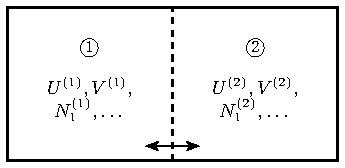
\includegraphics{figuras/pared-permeable.pdf}
\end{figure}
Entonces, las condiciones de cerradura para la energía y las partículas son
\begin{align*}
  U^{(1)}+U^{(2)}&=\text{cte.},\\
  N_1^{(1)}+N_1^{(2)}&=\text{cte.}
\end{align*}
Para este sistema cerrado se tiene que los cambios en $S$ para un proceso virtual adecuado es
$\dd S=0$, es decir,
\begin{align*}
  \dd S&=\pdvc{S}{U^{(1)}}{V^{(1)},N_1^{(1)},\dots}\dd U^{(1)}+\pdvc{S}{N_1^{(1)}}{U^{(1)},V^{(1)},\dots}\dd N_1^{(1)}\\
    &\quad+\pdvc{S}{U^{(2)}}{V^{(2)},N_1^{(2)},\dots}\dd U^{(2)}+\pdvc{S}{N_1^{(2)}}{U^{(2)},V^{(2)},\dots}\dd N_1^{(2)}\\
  &=\frac{1}{T^{(1)}}\dd U^{(1)}-\frac{\mu_1^{(1)}}{T^{(1)}}\dd N_1^{(1)}+\frac{1}{T^{(2)}}\dd U^{(2)}-\frac{\mu_1^{(2)}}{T^{(2)}}\dd N_1^{(2)}.
\end{align*}
Usando las condiciones de cerradura ($\dd U^{(2)}=-\dd U^{(1)}$, $\dd N_1^{(2)}=-\dd N_1^{(1)}$) e
igualando a cero se llega a
\begin{equation*}
  \left(\frac{1}{T^{(1)}}-\frac{1}{T^{(2)}}\right)\dd U^{(1)}-\left(\frac{\mu_1^{(1)}}{T^{(1)}}-\frac{\mu_1^{(2)}}{T^{(2)}}\right)\dd N_1^{(1)}=0,
\end{equation*}
y ya que este estado se alcanza cuando $\dd U^{(1)}$ y $\dd N_1^{(1)}$ se anulan (son independientes),
lo que implica que
\begin{equation*}
  \frac{1}{T^{(1)}}=\frac{1}{T^{(2)}},\quad\frac{\mu_1^{(1)}}{T^{(1)}}=\frac{\mu_1^{(2)}}{T^{(2)}}
  \qquad\text{o bien}\qquad
  \boxed{T^{(1)}=T^{(2)}}\quad\boxed{\mu_1^{(1)}=\mu_1^{(2)}}
\end{equation*}

Desde el punto de vista de las condiciones de equilibrio, la temperatura puede ser interpretada como
una especie de ``potencial'' del flujo de calor, ya que, como vimos, indica el sentido del flujo del
calor, desde sistemas de temperatura mayor hacia sistemas con una temperatura menor. Similarmente,
para el potencial químico, estas condiciones de equilibrio muestran que $\mu$ actúa como un
potencial ante el flujo de materia. Una diferencia en el potencial químico implica una fuerza
generalizada para el flujo de materia.

Para analizar la dirección del flujo de materia, tomemos la relación
\begin{equation*}
  \dd S=\left(\frac{1}{T^{(1)}}-\frac{1}{T^{(2)}}\right)\dd U^{(1)}-\left(\frac{\mu_1^{(1)}}{T^{(1)}}-\frac{\mu_1^{(2)}}{T^{(2)}}\right)\dd N_1^{(1)}.
\end{equation*}
Considerando $T^{(1)}=T^{(2)}=T$, el primer término se anula, por lo que
\begin{equation*}
  \dd S=\left(-\frac{\mu_1^{(1)}}{T}+\frac{\mu_1^{(2)}}{T}\right)\dd N_1^{(1)}=\frac{\mu_1^{(2)}-\mu_1^{(1)}}{T}\,\dd N_1^{(1)}.
\end{equation*}
Por lo tanto, si $\mu_1^{(1)}>\mu_1^{(2)}$, entonces $\dd N_1^{(1)}<0$ para que $\dd S>0$, por lo que
las partículas tenderán a fluir desde las regiones de mayor potencial químico hacia las regiones de
menor potencial químico. De ahí el nombre de \emph{potencial químico}.

\subsection*{Equilibrio químico}

Los sistemas que pasan por reacciones químicas guardan una fuerte similitud con los sistemas
difusivos recién presentados, los cuales son gobernados por las condiciones de equilibrio
expresadas en términos de $\mu$.

En una reacción química, el número de moles cambia: algunos se incrementan a expensas de la
disminución de otros. La relación entre este cambio de moles está gobernada por las ecuaciones de
las reacciones químicas, como
\begin{equation*}
  2\,\mathrm{H_2}+\mathrm{O_2}\rightleftharpoons2\,\mathrm{H_2O}
  \qquad\text{o}\qquad
  2\,\mathrm{O}\rightleftharpoons\mathrm{O_2}.
\end{equation*}
La primera ecuación indica que el cambio en el número de moles es en la razón $-2:-1:+2$ entre el
hidrógeno, el oxígeno y el agua.

De modo más general, se puede escribir la ecuación para una reacción química, para un sistema con
$r$ componentes, de la forma
\begin{equation*}
  0\rightleftharpoons\sum_{j=1}^{r}\nu_j A_j,
\end{equation*}
donde $\nu_j$ son los \textbf{coeficientes estequiométricos} y $A_j$ son los símbolos de los
componentes. Para el caso de la reacción del agua,
$\nu_1=-2$, $\nu_2=-1$, $\nu_3=+2$ y $A_1=\mathrm{H_2}$, $A_2=\mathrm{O_2}$, $A_3=\mathrm{H_2O}$, de
modo que
\begin{equation*}
  0\rightleftharpoons-2A_1-1A_2+2A_3.
\end{equation*}
Si la reacción se ve en sentido opuesto (disociación del agua en hidrógeno y oxígeno), los signos de
los $\nu_j$ se invierten, ya que estos son escogidos arbitrariamente.

Además, la relación fundamental del sistema es $S=S(U,V,N_1,N_2,\dots,N_r)$. Si en el curso de una
reacción química tanto $U$ como $V$ permanecen fijos, se considera que el sistema se encuentra
encerrado en un contenedor rígido y adiabático para la reacción (no es el más común tipo de
frontera química; usualmente son abiertos y permiten el intercambio de energía con la atmósfera y
el cambio de volumen). El cambio de entropía en tal proceso químico virtual es
% NOTA: el manuscrito dice "El cambio de energía en tal proceso químico virtual"; la expresión que sigue es dS, por lo que se escribió "entropía".
\begin{equation*}
  \dd S=-\sum_{j=1}^{r}\frac{\mu_j}{T}\,\dd N_j.
\end{equation*}
Pero, de acuerdo con lo anteriormente visto, los cambios en el número de moles deben ser
proporcionales a los coeficientes estequiométricos $\nu_j$. Por simplicidad consideramos
$\dd N_j\propto\nu_j$, es decir, $\dd N_j=\nu_j\,\dd\tilde{N}$, donde $\dd\tilde{N}$ es el factor de
proporcionalidad. Entonces el cambio en la entropía es
\begin{equation*}
  \dd S=-\frac{\dd\tilde{N}}{T}\sum_{j=1}^{r}\mu_j\nu_j,
\end{equation*}
y de acuerdo con el postulado II la entropía tiene que ser un máximo en el estado de equilibrio, de
modo que
\begin{equation*}
  \dd S=0=-\frac{\dd\tilde{N}}{T}\sum_{j=1}^{r}\mu_j\nu_j
  \qquad\therefore\qquad
  \boxed{\sum_{j=1}^{r}\mu_j\nu_j=0}\quad\text{(condición de equilibrio químico)}.
\end{equation*}
Si se conocen las ecuaciones de estado de la mezcla, las condiciones de equilibrio químico permiten
encontrar una solución explícita para el número final de moles.

Por ejemplo, si se introduce hidrógeno, oxígeno y dióxido de carbono en un recipiente, las
siguientes reacciones químicas pueden ocurrir:
\begin{itemize}[itemsep=0pt]
  \item $\mathrm{H_2}+\tfrac{1}{2}\mathrm{O_2}\rightleftharpoons\mathrm{H_2O}$,
  \item $\mathrm{CO_2}+\mathrm{H_2}\rightleftharpoons\mathrm{CO}+\mathrm{H_2O}$,
  \item $\mathrm{CO}+\tfrac{1}{2}\mathrm{O_2}\rightleftharpoons\mathrm{CO_2}$.
\end{itemize}

En el equilibrio se tienen (despejando):
\begin{align}
  \mu_{\mathrm{H_2}}+\tfrac{1}{2}\mu_{\mathrm{O_2}}&=\mu_{\mathrm{H_2O}},\tag{1}\\
  \mu_{\mathrm{CO_2}}+\mu_{\mathrm{H_2}}&=\mu_{\mathrm{CO}}+\mu_{\mathrm{H_2O}},\tag{2}\\
  \mu_{\mathrm{CO}}+\tfrac{1}{2}\mu_{\mathrm{O_2}}&=\mu_{\mathrm{CO_2}}.\tag{3}
\end{align}
Son dos ecuaciones independientes: la (1) es la suma neta de (2) y (3).

\subsection*{Ejercicios}

\begin{ejercicio}[P.\,2.6.3]
  Dos sistemas particulares tienen las siguientes ecuaciones de estado:
  \begin{equation*}
    \frac{1}{T^{(1)}}=\frac{3}{2}R\,\frac{N^{(1)}}{U^{(1)}}
    \qquad\text{y}\qquad
    \frac{1}{T^{(2)}}=\frac{5}{2}R\,\frac{N^{(2)}}{U^{(2)}},
  \end{equation*}
  donde $R$ es la constante universal de los gases. El número de moles del primer sistema es
  $N^{(1)}=2$ y el del segundo sistema es $N^{(2)}=3$. Los dos sistemas están separados por una
  pared diatérmica y la energía total del sistema es $2.5\times10^{3}\ \mathrm{J}$. ¿Cuál es la
  energía interna de cada sistema en equilibrio?
\end{ejercicio}

\begin{solucion}
  En condiciones de equilibrio, el sistema está en equilibrio térmico por lo establecido en el
  problema; entonces $1/T^{(1)}=1/T^{(2)}$, lo que implica que
  \begin{equation*}
    \frac{3}{2}R\,\frac{N^{(1)}}{U^{(1)}}=\frac{5}{2}R\,\frac{N^{(2)}}{U^{(2)}}
    \quad\Longrightarrow\quad
    \frac{3(2)}{U^{(1)}}=\frac{5(3)}{U^{(2)}}
    \quad\Longrightarrow\quad
    \frac{2}{U^{(1)}}=\frac{5}{U^{(2)}}
    \quad\Longrightarrow\quad
    2U^{(2)}=5U^{(1)}.
  \end{equation*}
  Asimismo, sabemos que $U^{(1)}+U^{(2)}=\text{cte.}=2.5\times10^{3}\ \mathrm{J}$. Sustituyendo
  $U^{(2)}=\frac{5}{2}U^{(1)}$,
  \begin{equation*}
    U^{(1)}+\frac{5}{2}U^{(1)}=\frac{7}{2}U^{(1)}=2.5\times10^{3}\ \mathrm{J}
    \quad\Longrightarrow\quad
    \boxed{U^{(1)}=\frac{2}{7}\left(2.5\times10^{3}\ \mathrm{J}\right)=714.28\ \mathrm{J}}
  \end{equation*}
  y
  \begin{equation*}
    \boxed{U^{(2)}=\frac{5}{2}U^{(1)}=\frac{5}{2}\left(714.28\ \mathrm{J}\right)=1785.71\ \mathrm{J}}
  \end{equation*}
\end{solucion}

\begin{ejercicio}[P.\,2.7.1]
  Tres cilindros son ajustados con $4$ pistones, tal como muestra la figura siguiente. Las áreas de
  las secciones transversales están en la razón $A_1:A_2:A_3=1:2:3$. Pares de pistones son acoplados
  de tal modo que sus desplazamientos (movimientos lineales) son iguales. Las paredes de los
  cilindros son diatérmicas y están conectadas por una barra conductora del calor (mostrada con las
  líneas cruzadas en la figura). El sistema entero está aislado (de manera que, por ejemplo, no hay
  presión ejercida en las paredes externas de los pistones). Encuentre las razones de las presiones
  en los tres cilindros.
  \begin{figure}[H]
    \centering
    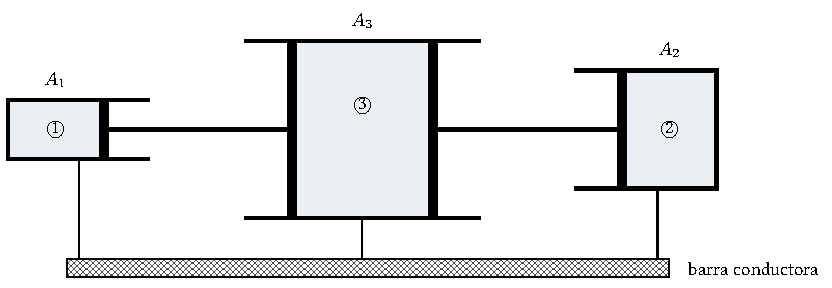
\includegraphics{figuras/tres-cilindros.pdf}
  \end{figure}
\end{ejercicio}

\begin{solucion}
  La condición de cerradura del sistema respecto a la energía se deriva de la conservación de la
  energía, $U^{(1)}+U^{(2)}+U^{(3)}=\text{cte.}$, por lo que para una transferencia virtual
  \begin{equation*}
    \delta U^{(1)}+\delta U^{(2)}+\delta U^{(3)}=0
    \qquad\text{o}\qquad
    \delta U^{(3)}=-\delta U^{(1)}-\delta U^{(2)}.
  \end{equation*}
  La segunda condición de cerradura se deriva del volumen total del sistema y de las proporciones
  indicadas en el problema, $1:2:3$: si el volumen aumenta en \textcircled{3} (se expande), entonces
  tanto $V^{(1)}$ como $V^{(2)}$ disminuyen, de acuerdo con la proporción $1:2:3$ de las áreas
  $A_1:A_2:A_3$; por lo que una expansión (movimientos iguales) en $V^{(3)}$ implica una reducción
  tanto en $V^{(1)}$ como en $V^{(2)}$, con lo que $\delta V_{\mathrm{tot}}=0$. Al ser
  desplazamientos iguales, $\delta V=A\,\delta h$; pero $\delta h$ es igual para todos los cilindros:
  \begin{align*}
    \delta V^{(3)}&=A_3\,\delta h=3A_1\,\delta h=3\,\delta V^{(1)},\\
    \delta V^{(2)}&=A_2\,\delta h=2A_1\,\delta h=2\,\delta V^{(1)},
  \end{align*}
  relacionando, $\delta V^{(3)}=\frac{3}{2}\,\delta V^{(2)}$. Por lo tanto
  \begin{equation*}
    \delta V_{\mathrm{tot}}=0=\delta V^{(3)}+3\,\delta V^{(1)}+\tfrac{3}{2}\,\delta V^{(2)}
    \qquad\text{o}\qquad
    \delta V^{(3)}=-3\,\delta V^{(1)}-\tfrac{3}{2}\,\delta V^{(2)}
  \end{equation*}
  (si se toma en sentido contrario solo cambia un signo global).
  % REVISAR (manuscrito): la relación \delta V^{(3)}=-3\delta V^{(1)}-\frac{3}{2}\delta V^{(2)} es correcta cuando cada par de pistones se desplaza de forma independiente (\delta V^{(3)} recibe la contribución de los dos pares: -(A_3/A_1)\delta V^{(1)} y -(A_3/A_2)\delta V^{(2)}); con un único \delta h común no sería consistente con \delta V_tot=0. El resultado final (6:3:2) coincide con esa lectura.
  Por lo que los cambios en la entropía en un proceso virtual son
  \begin{equation*}
    \delta S=\frac{1}{T^{(1)}}\delta U^{(1)}+\frac{1}{T^{(2)}}\delta U^{(2)}+\frac{1}{T^{(3)}}\delta U^{(3)}
      +\frac{P^{(1)}}{T^{(1)}}\delta V^{(1)}+\frac{P^{(2)}}{T^{(2)}}\delta V^{(2)}+\frac{P^{(3)}}{T^{(3)}}\delta V^{(3)},
  \end{equation*}
  y como se debe cumplir que $\delta S=0$, se puede sustituir para simplificar, eliminando
  $\delta U^{(3)}$ y $\delta V^{(3)}$:
  \begin{align*}
    0&=\frac{1}{T^{(1)}}\delta U^{(1)}+\frac{1}{T^{(2)}}\delta U^{(2)}+\frac{1}{T^{(3)}}\left(-\delta U^{(1)}-\delta U^{(2)}\right)\\
     &\quad+\frac{P^{(1)}}{T^{(1)}}\delta V^{(1)}+\frac{P^{(2)}}{T^{(2)}}\delta V^{(2)}+\frac{P^{(3)}}{T^{(3)}}\left(-3\,\delta V^{(1)}-\tfrac{3}{2}\,\delta V^{(2)}\right)\\
     &=\left(\frac{1}{T^{(1)}}-\frac{1}{T^{(3)}}\right)\delta U^{(1)}+\left(\frac{1}{T^{(2)}}-\frac{1}{T^{(3)}}\right)\delta U^{(2)}\\
     &\quad+\left(\frac{P^{(1)}}{T^{(1)}}-3\,\frac{P^{(3)}}{T^{(3)}}\right)\delta V^{(1)}+\left(\frac{P^{(2)}}{T^{(2)}}-\frac{3}{2}\,\frac{P^{(3)}}{T^{(3)}}\right)\delta V^{(2)}.
  \end{align*}
  Para que se cumpla que $\delta S=0$, todos los coeficientes se deben anular, porque como
  $\delta U^{(1)}$, $\delta U^{(2)}$, $\delta V^{(1)}$ y $\delta V^{(2)}\neq0$ son independientes:
  \begin{equation*}
    \frac{1}{T^{(1)}}=\frac{1}{T^{(3)}},\quad\frac{1}{T^{(2)}}=\frac{1}{T^{(3)}}
    \qquad\text{y}\qquad
    \frac{P^{(1)}}{T^{(1)}}=3\,\frac{P^{(3)}}{T^{(3)}},\quad\frac{P^{(2)}}{T^{(2)}}=\frac{3}{2}\,\frac{P^{(3)}}{T^{(3)}},
  \end{equation*}
  o bien, como las temperaturas son iguales,
  \begin{equation*}
    \boxed{P^{(1)}=3P^{(3)}\quad\text{y}\quad2P^{(2)}=3P^{(3)}}
  \end{equation*}
  es decir, $P^{(1)}:P^{(2)}:P^{(3)}=6:3:2$.
\end{solucion}

\begin{ejercicio}[P.\,2.8.1]
  La ecuación fundamental de un sistema particular de dos componentes es
  \begin{equation*}
    S=NA+NR\ln\frac{U^{3/2}V}{N^{5/2}}-N_1R\ln\frac{N_1}{N}-N_2R\ln\frac{N_2}{N},
    \qquad N\equiv N_1+N_2,
  \end{equation*}
  donde $A$ es una constante no especificada. Un cilindro rígido cerrado de volumen total de $10$
  litros se divide en dos cámaras de volumen igual por una membrana rígida diatérmica, permeable al
  primer tipo $N_1$ pero impermeable a $N_2$. En una cámara se coloca una muestra del sistema con
  parámetros originales $N_1^{(1)}=0.5$, $N_2^{(1)}=0.75$, $V^{(1)}=5$ litros y $T^{(1)}=300\ \mathrm{K}$.
  En la segunda cámara se coloca una muestra del mismo sistema con parámetros originales
  $N_1^{(2)}=1$, $N_2^{(2)}=0.5$, $V^{(2)}=5$ litros y $T^{(2)}=250\ \mathrm{K}$. Después de que se
  establece el equilibrio, ¿cuáles son los valores de $N_1^{(1)}$, $N_1^{(2)}$, $T$, $P^{(1)}$ y
  $P^{(2)}$?
\end{ejercicio}

\begin{solucion}
  Derivando para obtener la temperatura y la presión (recordando que $\pdv{\ln x}{x}=\frac{1}{x}$):
  \begin{align*}
    \frac{1}{T}&=\pdvc{S}{U}{V,N_1,N_2}=NR\,\frac{3}{2}\,\frac{1}{U}=\frac{3}{2}\,\frac{NR}{U},\\
    \frac{P}{T}&=\pdvc{S}{V}{U,N_1,N_2}=NR\,\frac{1}{V}=\frac{NR}{V}.
  \end{align*}
  Para el potencial químico, escribiendo $S=(N_1+N_2)A+(N_1+N_2)R\ln\frac{U^{3/2}V}{(N_1+N_2)^{5/2}}-N_1R\ln\frac{N_1}{N_1+N_2}-N_2R\ln\frac{N_2}{N_1+N_2}$,
  derivando respecto a $N_i$ (usando $\partial N/\partial N_i=1$) se obtiene
  \begin{equation*}
    \pdvc{S}{N_i}{U,V,N_j}=A-\frac{5}{2}R+R\ln\frac{U^{3/2}V}{N_i\,N^{3/2}},\qquad i=1,2,
  \end{equation*}
  de modo que
  \begin{equation*}
    \frac{\mu_i}{T}=-\pdvc{S}{N_i}{U,V,N_j}=-\left[R\ln\frac{U^{3/2}V}{N_i\,N^{3/2}}+\left(A-\frac{5}{2}R\right)\right].
  \end{equation*}
  % NOTA: el manuscrito escribe \mu_1/T=-[A+R\ln(\cdots)+\frac{5}{2}R-R\ln(N_1/N)] y \mu/T=R\ln(\cdots)+[A-\frac{5}{2}R] (sin el signo global); tras derivar, el término constante es -\frac{5}{2}R y el signo global es "-". Esto no afecta el resultado de equilibrio (la igualdad de \mu_1/T entre las cámaras es insensible al signo).
  Aplicando las condiciones de equilibrio, $1/T^{(1)}=1/T^{(2)}$:
  \begin{equation*}
    \frac{3}{2}R\,\frac{N_1^{(1)}+N_2^{(1)}}{U^{(1)}}=\frac{3}{2}R\,\frac{N_1^{(2)}+N_2^{(2)}}{U^{(2)}}
    \quad\Longrightarrow\quad
    \frac{N_1^{(1)}+N_2^{(1)}}{U^{(1)}}=\frac{N_1^{(2)}+N_2^{(2)}}{U^{(2)}},
  \end{equation*}
  y $\mu_1^{(1)}/T^{(1)}=\mu_1^{(2)}/T^{(2)}$ implica
  \begin{equation*}
    \ln\frac{\bigl(U^{(1)}\bigr)^{3/2}V^{(1)}}{N_1^{(1)}\bigl[N_1^{(1)}+N_2^{(1)}\bigr]^{3/2}}
    =\ln\frac{\bigl(U^{(2)}\bigr)^{3/2}V^{(2)}}{N_1^{(2)}\bigl[N_1^{(2)}+N_2^{(2)}\bigr]^{3/2}}.
  \end{equation*}
  Tomando esta igualdad, con $V^{(1)}=V^{(2)}$, y comparando con la relación de temperaturas
  (elevada a la potencia $3/2$),
  \begin{equation*}
    \frac{\bigl[N_1^{(1)}+N_2^{(1)}\bigr]^{3/2}}{\bigl(U^{(1)}\bigr)^{3/2}}=\frac{\bigl[N_1^{(2)}+N_2^{(2)}\bigr]^{3/2}}{\bigl(U^{(2)}\bigr)^{3/2}}
    \quad\Longrightarrow\quad
    N_1^{(1)}=N_1^{(2)},
  \end{equation*}
  y como $N_1^{(1)}+N_1^{(2)}=0.5+1=1.5$, se tiene $\boxed{N_1^{(1)}=N_1^{(2)}=0.75}$.

  Para encontrar las energías, tenemos la derivada $\dfrac{1}{T}=\dfrac{3}{2}\dfrac{NR}{U}$, o bien
  $U=\dfrac{3}{2}NRT$. Por lo tanto, las energías iniciales son
  \begin{align*}
    U^{(1)}&=\frac{3}{2}N^{(1)}RT^{(1)}=\frac{3}{2}\left(N_1^{(1)}+N_2^{(1)}\right)RT^{(1)}=\frac{3}{2}(0.5+0.75)R\,(300\ \mathrm{K})=562.5\,R\ \mathrm{K},\\
    U^{(2)}&=\frac{3}{2}N^{(2)}RT^{(2)}=\frac{3}{2}\left(N_1^{(2)}+N_2^{(2)}\right)RT^{(2)}=\frac{3}{2}(1+0.5)R\,(250\ \mathrm{K})=562.5\,R\ \mathrm{K}.
  \end{align*}

  Las energías finales serán entonces $U^{(1)}=\frac{3}{2}N^{(1)}RT$ y $U^{(2)}=\frac{3}{2}N^{(2)}RT$, con
  $N^{(1)}=N_1^{(1)}+N_2^{(1)}=0.75+0.75=1.5$ y $N^{(2)}=N_1^{(2)}+N_2^{(2)}=0.75+0.5=1.25$ (el
  número de moles de $N_2$ no cambia en cada cámara, ya que la membrana es impermeable a él). Así,
  \begin{equation*}
    U^{(1)}=\frac{3}{2}R(1.5)T,\qquad U^{(2)}=\frac{3}{2}R(1.25)T
    \quad\Longrightarrow\quad
    U^{(1)}+U^{(2)}=4.125\,RT,
  \end{equation*}
  % NOTA: el manuscrito escribe "N=1.5" y (1.5) en ambas cámaras; los valores que dan 4.125RT, T=272.7 K, P^{(1)}=6.8e5 Pa y P^{(2)}=5.7e5 Pa corresponden a N^{(1)}=1.5 y N^{(2)}=1.25, que es lo que se usa aquí.
  y comparando con las iniciales (la energía total se conserva),
  \begin{equation*}
    4.125\,RT=2(562.5\,R)\quad\Longrightarrow\quad\boxed{T=272.7\ \mathrm{K}}
  \end{equation*}
  Con $PV=NRT$ (usando $R=8.314\ \mathrm{J/(mol\,K)}$ y $V^{(1)}=V^{(2)}=5\ \mathrm{L}$):
  \begin{align*}
    P^{(1)}V^{(1)}&=N^{(1)}RT\quad\Longrightarrow\quad\boxed{P^{(1)}=6.8\times10^{5}\ \mathrm{Pa}},\\
    P^{(2)}V^{(2)}&=N^{(2)}RT\quad\Longrightarrow\quad\boxed{P^{(2)}=5.7\times10^{5}\ \mathrm{Pa}}.
  \end{align*}
\end{solucion}

